\subsubsection{Reator do Tipo \textit{PFR}}

Um reator tubular é caracterizado por escoamento pistonado, sem mistura axial significativa: cada elemento de fluido que entra percorre o reator como se fosse um reator batelada em movimento, evoluindo em conversão conforme o comprimento.

Para uma conversão alvo $X$, o volume requerido de um \textit{PFR} ideal é dado pela integração da equação de \textit{design} diferencial ao longo da conversão \cite{levenspiel2000}. Matematicamente:

\begin{equation}
V = {( R + 1 ) \cdot F}_{A 0} \cdot \int_{\frac{R}{R + 1} X \ }^{X} \frac{d X}{- r_{A}}
\label{eq:pfr_design}
\end{equation}

Tendo que $R$ representa a razão de reagentes não limitantes inertes em relação ao limitante (se houver variação de vazão volumétrica) e o termo $( R + 1 )$ acomoda a variação de vazão na integração. No código, essa integral é avaliada numericamente (por exemplo, via \textit{scipy.integrate.quad}). Para o caso inverso, em que $V$ é conhecido e se busca $X$, utiliza-se novamente um procedimento iterativo (método de Brent) aplicando a equação de \textit{design} diferencial até encontrar a conversão cujo volume calculado corresponda ao especificado \cite{fogler2009}.

Considerando a similaridade estrutural e semântica com as rotinas de cálculo do \textit{CSTR}, destaca-se a diferença na função objetivo usada para o cálculo de volume, representada na Figura a seguir.

\begin{figure}[H]
    \centering
    \caption{Código da função objetivo para o \textit{PFR}}
    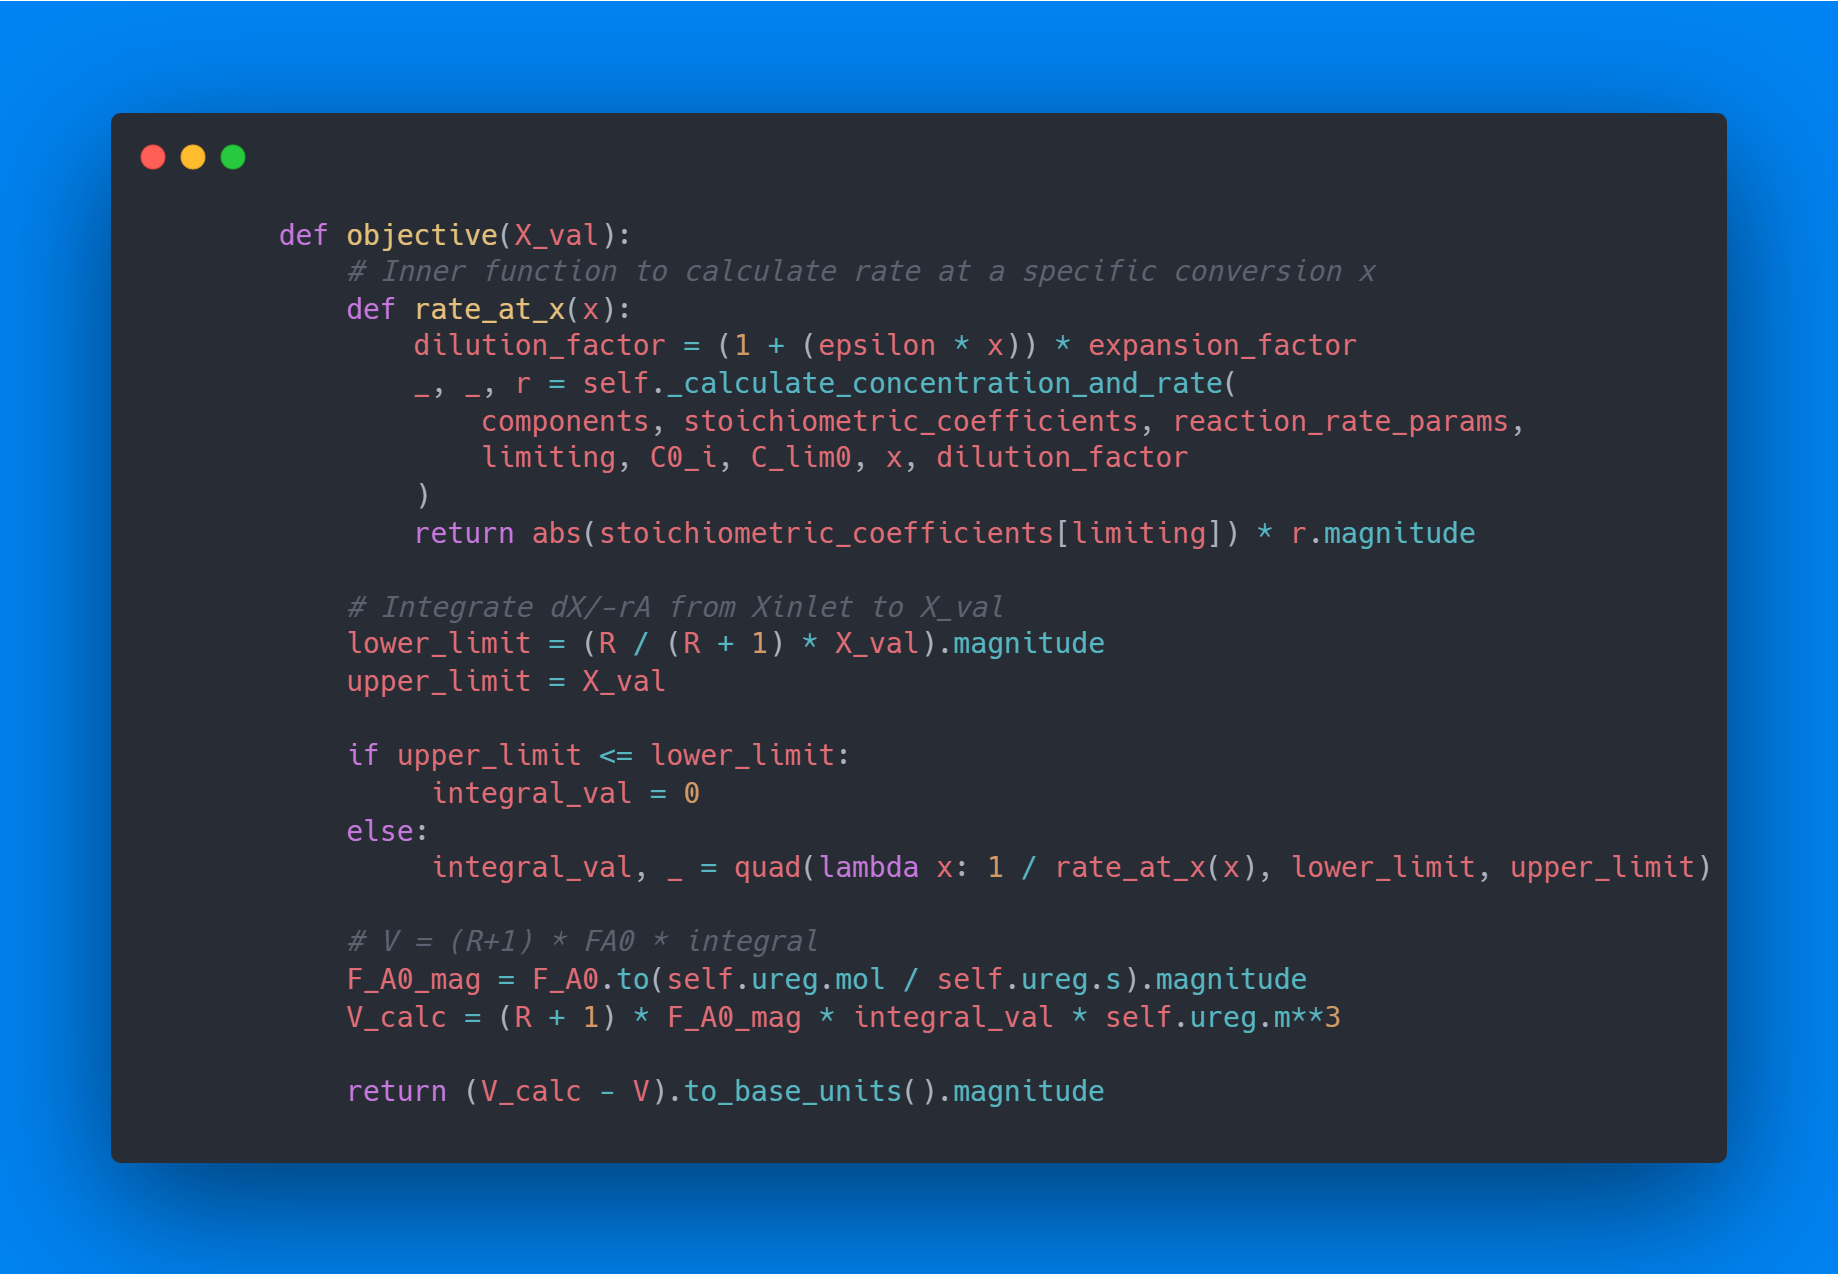
\includegraphics[width=\linewidth]{media/cap4_funcao_objetivo_pfr.png}
    \fonte{Elaboração própria (2026).}
\end{figure}

\subsection{Tubulações}

Para um correto cálculo de perdas de carga e seleção de bombas, o \textit{software} incorpora dados de catálogo de tubulações, rugosidades de materiais e comprimentos equivalentes de acessórios.

\textbf{Rugosidade de materiais.} A rugosidade absoluta do material interno do tubo influencia o fator de atrito em regime turbulento por meio da rugosidade relativa $\varepsilon/D$. Materiais metálicos, plásticos ou com incrustações apresentam valores típicos de rugosidade tabelados \cite{white2018}. Com o tempo de operação, depósitos e corrosão podem elevar a rugosidade efetiva, devendo-se considerar fatores de segurança.

\textbf{Catálogo de diâmetros.} São armazenadas dimensões padrão de tubulações (diâmetro externo, espessura e diâmetro interno resultante) para diferentes \textit{schedules} (por exemplo, SCH 10, 40 e 80) e materiais. Também podem ser incluídos dados de pressão máxima de trabalho e peso por metro. Isso permite que, dado um diâmetro calculado, o programa selecione o diâmetro nominal comercial mais próximo disponível.

\begin{figure}[H]
    \centering
    \caption{Especificações internas para tubulações}
    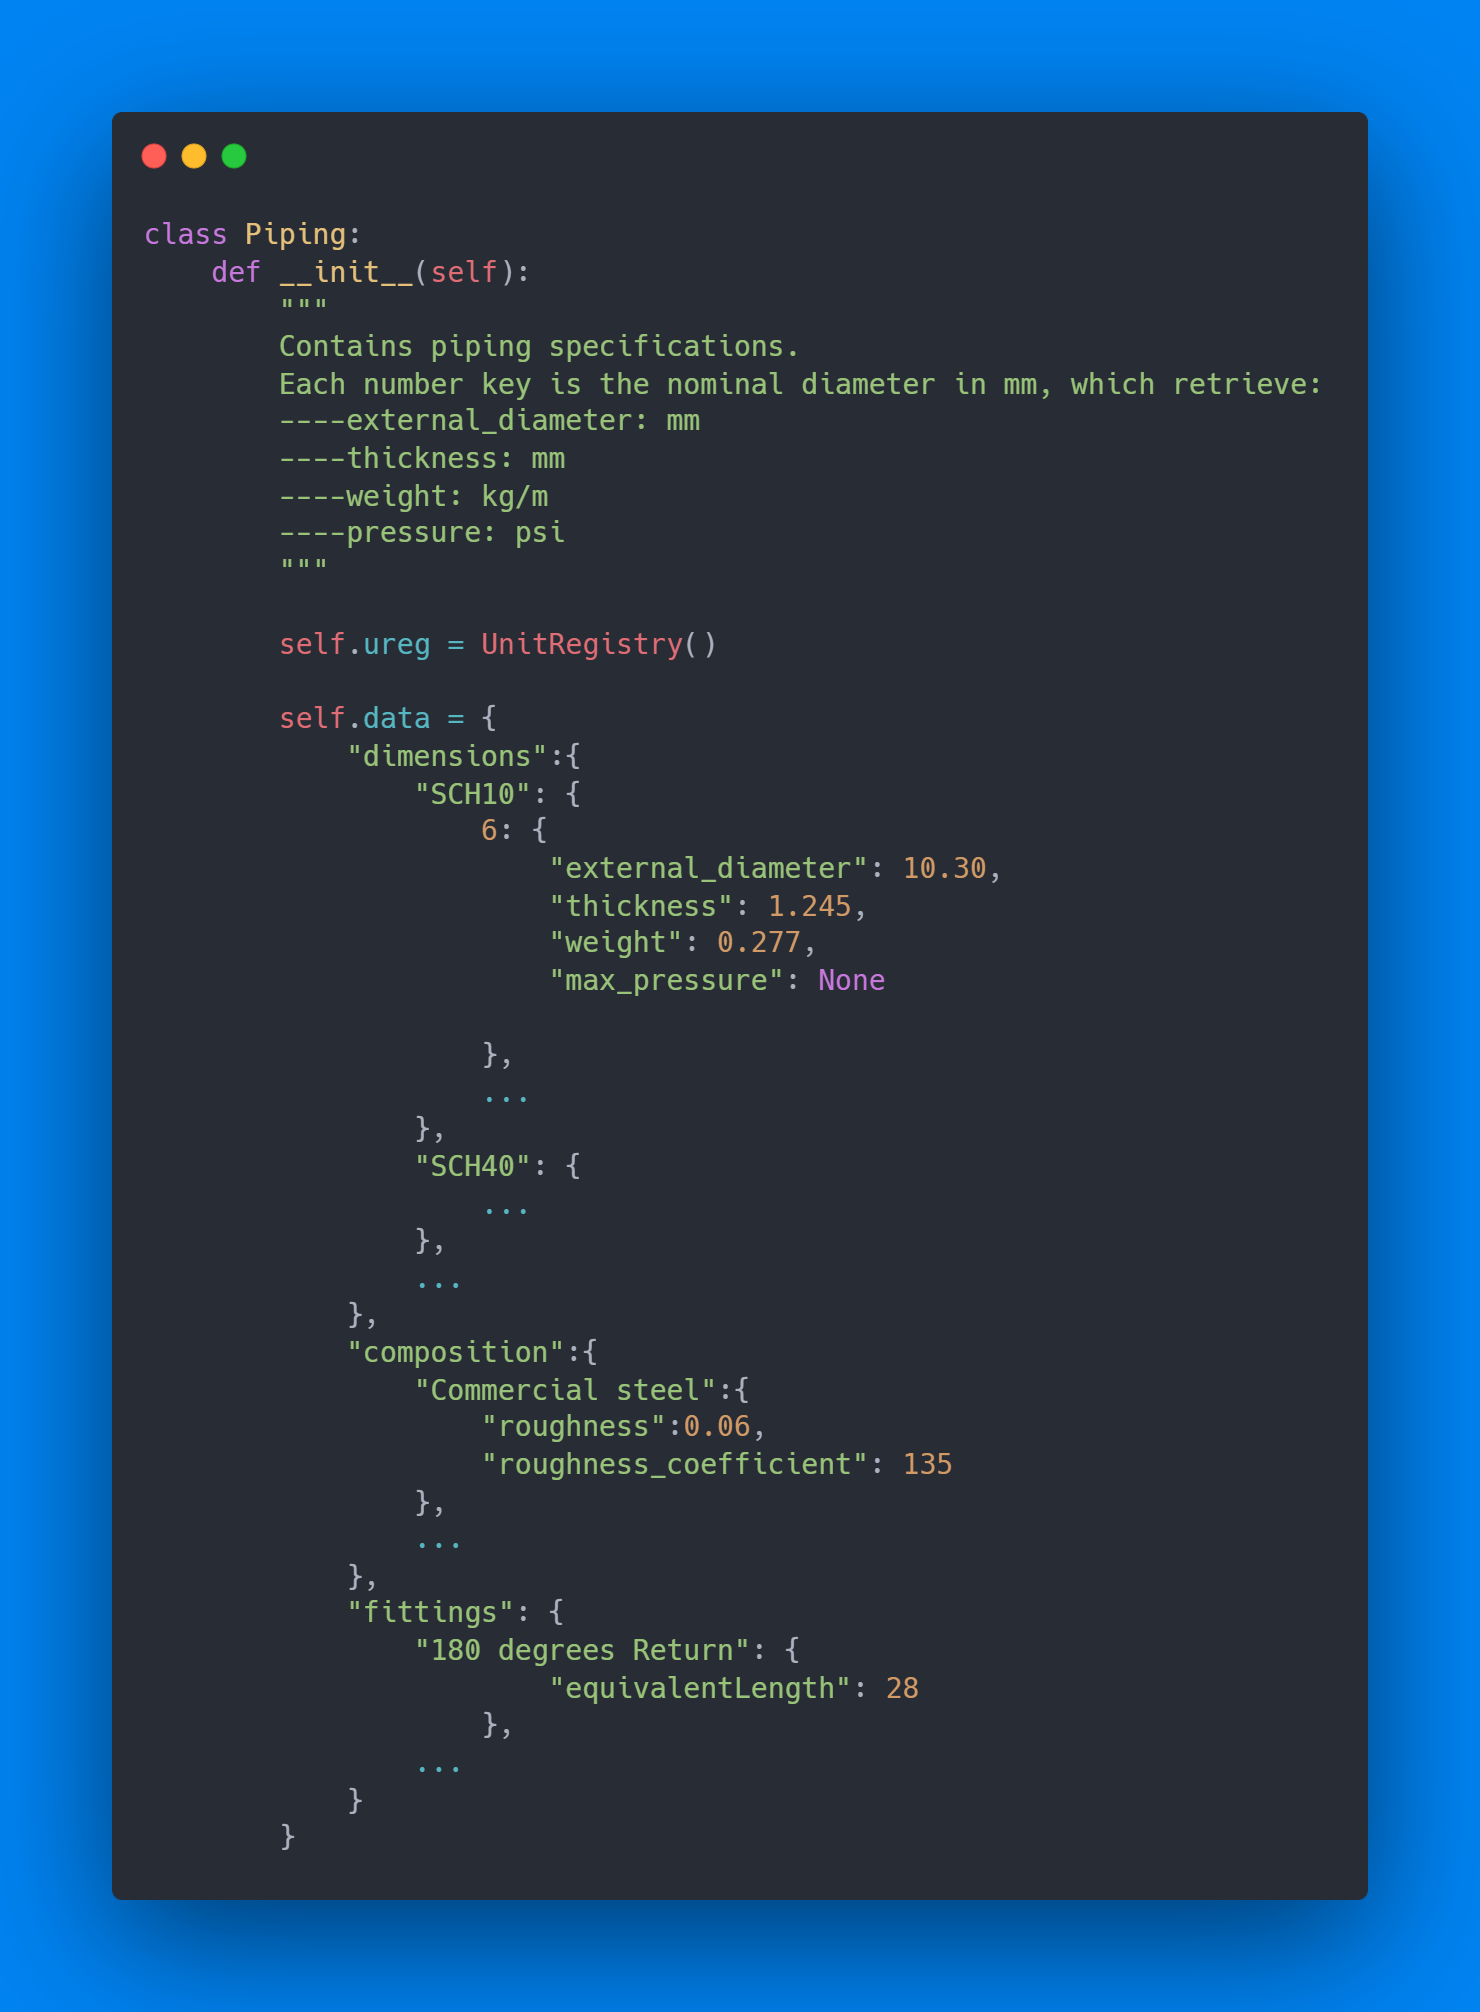
\includegraphics[width=\linewidth]{media/cap4_especificacoes_tubulacoes_hardcoded.png}
    \fonte{Elaboração própria (2026).}
\end{figure}

\textbf{Coeficientes de perda em acessórios.} Curvas, válvulas, expansões, contrações e conexões diversas introduzem perdas de carga locais. No modelo implementado, cada acessório pode ser contabilizado por um comprimento equivalente $L_{eq}$ ou por um fator adimensional de perda $K$. O comprimento equivalente total da tubulação é obtido pela soma dos acessórios e acrescentado ao comprimento linear. Esses dados, como fatores $K$ ou $L_{eq}$ típicos para cada acessório padrão, foram compilados de literatura de engenharia de escoamento \cite{perry2007}.

No cálculo de perdas de carga totais, o comprimento $L$ da tubulação reta é acrescido do comprimento equivalente $\sum_{}^{} L_{eq}$ das singularidades presentes. Uma estimativa inadequada da rugosidade ou do efeito de acessórios pode produzir erros significativos na previsão de perda de carga, resultando em superdimensionamento ou subdimensionamento de bombas. Assim, o uso de dados acurados de catálogo e correlações de atrito é fundamental para a confiabilidade do dimensionamento. A Figura a seguir exemplifica o cálculo da perda de carga por Darcy--Weisbach utilizando acessórios.

\begin{figure}[H]
    \centering
    \caption{Cálculo da perda de carga por Darcy--Weisbach com acessórios}
    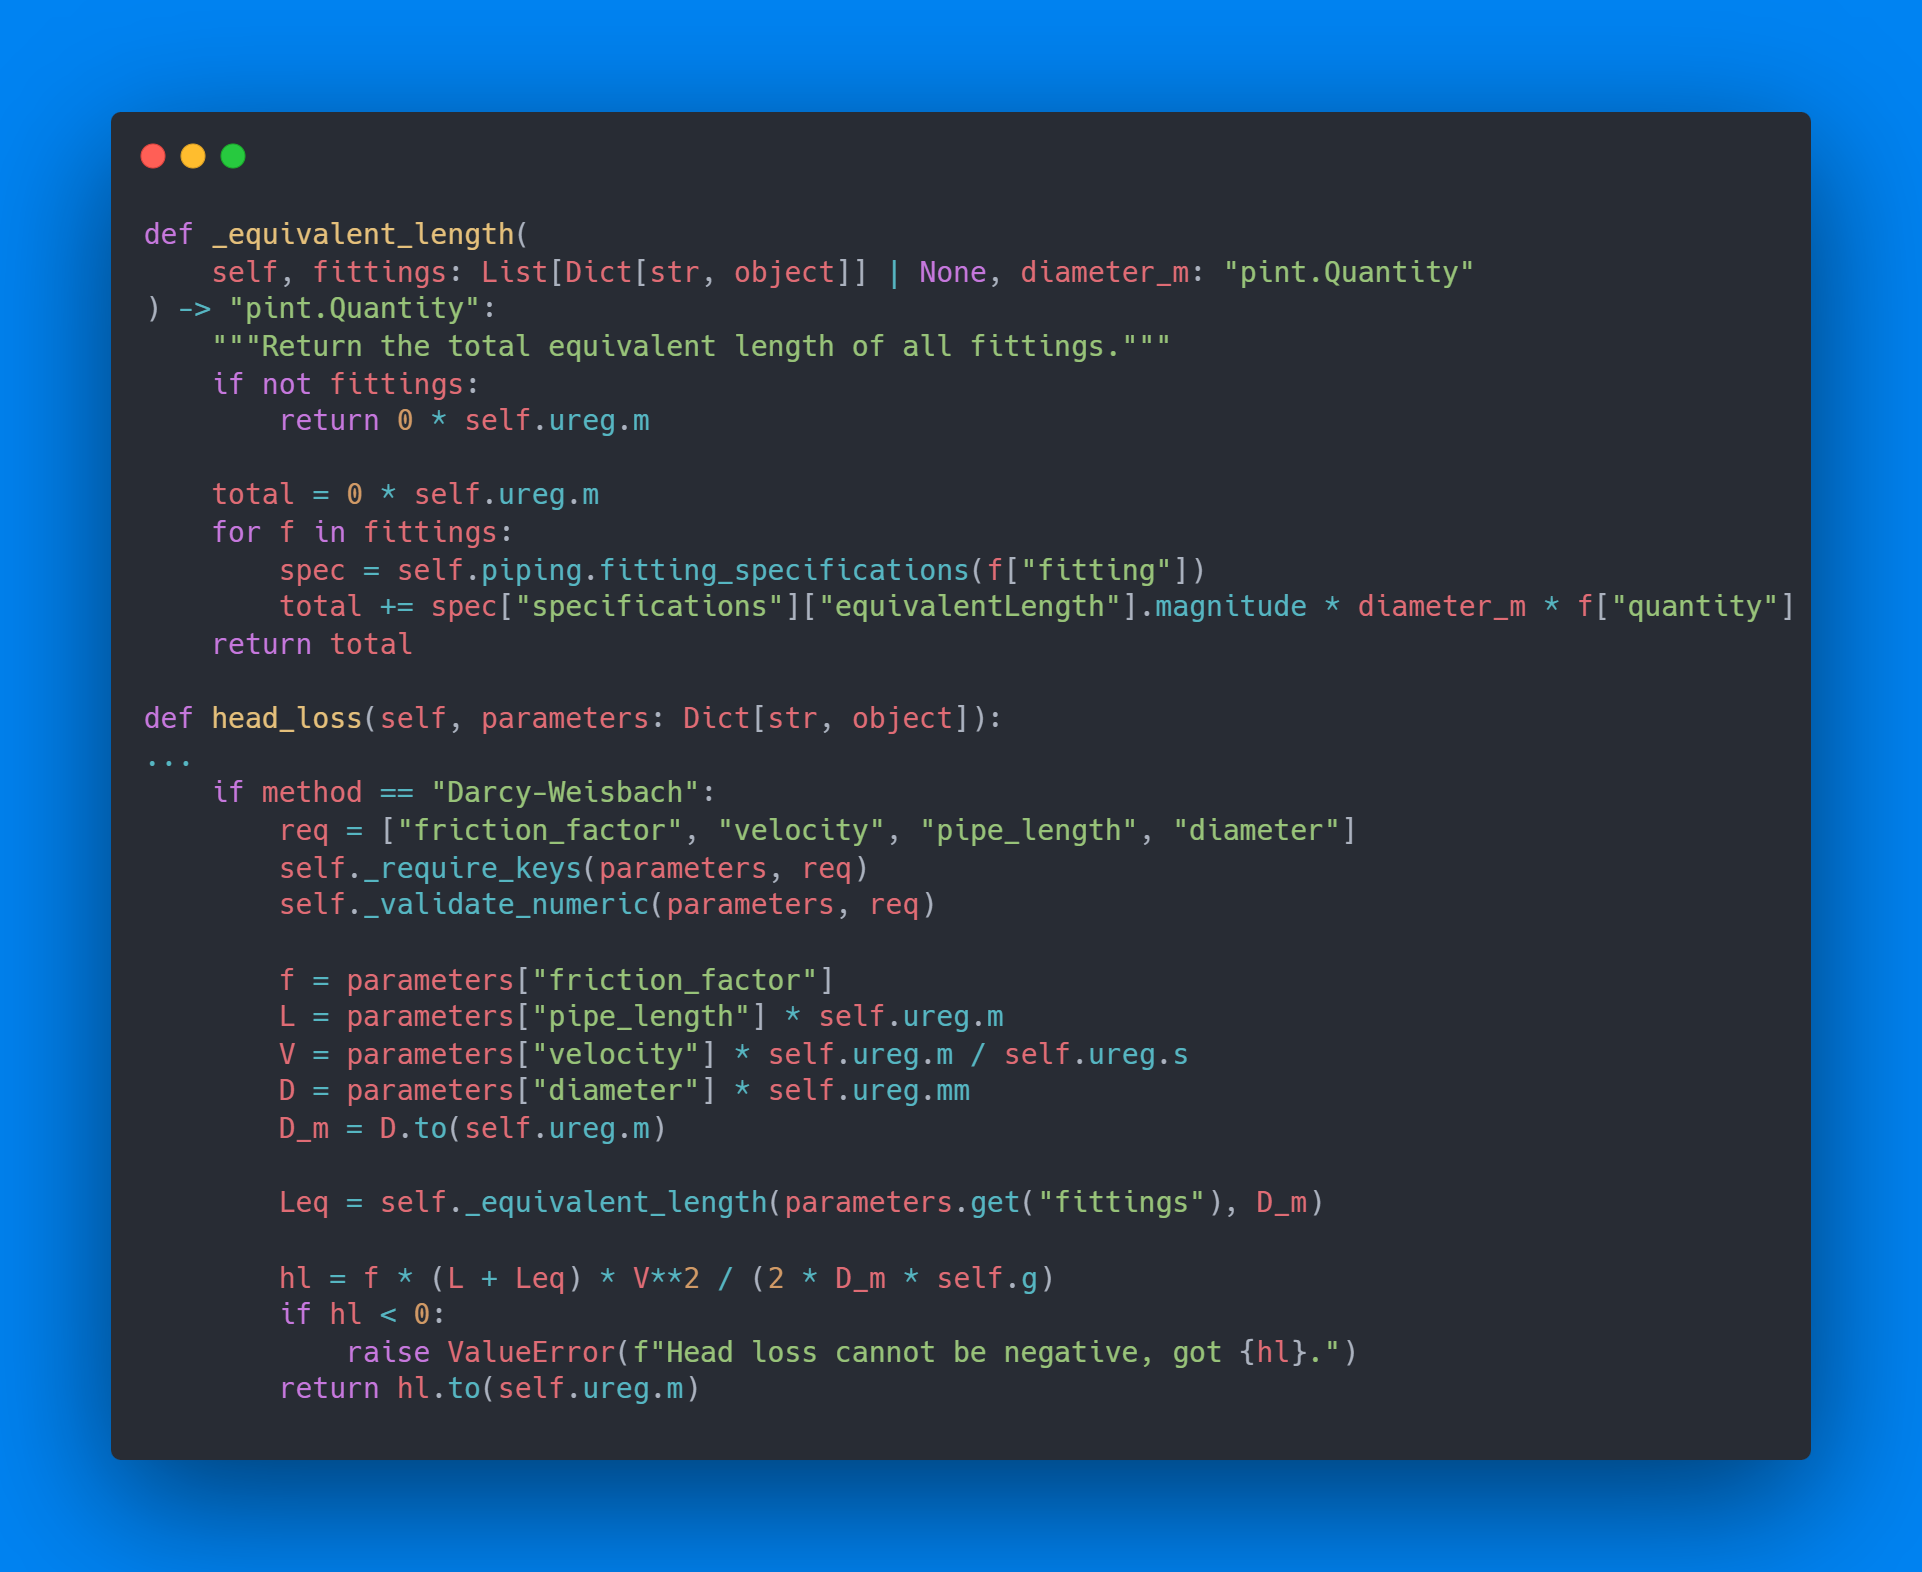
\includegraphics[width=\linewidth]{media/cap4_perda_carga_darcy_weisbach_acessorios.png}
    \fonte{Elaboração própria (2026).}
\end{figure}

\subsection{Balanço de Massa}

O balanço de massa aplica o princípio da conservação da massa a sistemas de processo: em regime estacionário, a massa que entra em um sistema deve ser igual à massa que sai, ajustada pela geração ou consumo devido a reações químicas \cite{felder2005}. Para cada componente, a quantidade produzida ou consumida deve ser contabilizada segundo a estequiometria.

\begin{equation}
\text{Acúmulo} = \text{Entradas} - \text{Saídas} + \text{Geração} - \text{Consumo}
\label{eq:mass_balance_word}
\end{equation}

No estado estacionário sem reação, o acúmulo é zero, de modo que:

\begin{equation}
\sum \dot{m}_{\mathrm{entrada}} = \sum \dot{m}_{\mathrm{saida}}
\label{eq:steady_state_mass_balance}
\end{equation}

Por componente $i$, incluindo reação química:

\begin{equation}
\sum \left(\dot{m}_{\mathrm{entrada},i} + \dot{m}_{\mathrm{geracao},i}\right) = \sum \left(\dot{m}_{\mathrm{saida},i} + \dot{m}_{\mathrm{consumo},i}\right)
\label{eq:component_mass_balance_rxn}
\end{equation}

Em que:
\begin{itemize}
    \item $\dot{m}$ é a vazão mássica.
\end{itemize}

Em problemas industriais, frequentemente há reciclo e purgas envolvidos nos balanços. Nesses casos, para divisores de fluxo (\textit{splitters}), define-se por exemplo:

\begin{equation}
F_{R} = f \cdot F_{P}
\label{eq:recycle_flow}
\end{equation}

\begin{equation}
F_{G} = ( 1 - f ) \cdot F_{P}
\label{eq:gross_product_flow}
\end{equation}

Em que:
\begin{itemize}
    \item $f$ é a fração de reciclo;
    \item $F_{G}$ é a vazão total do produto bruto;
    \item $F_{R}$ é a vazão do reciclo;
    \item $F_{P}$ é a vazão da purga.
\end{itemize}

Esses parâmetros permitem fechar balanços em sistemas com recirculação e calcular a acumulação de inertes ou subprodutos. Na Figura \ref{fig:mass_balance_results}, é apresentado o resultado gerado pelo \textit{software} para um balanço de massa contendo reciclo e reação.

\begin{figure}[H]
    \centering
    \caption{Resultados do balanço de massa com reciclo e reação}
    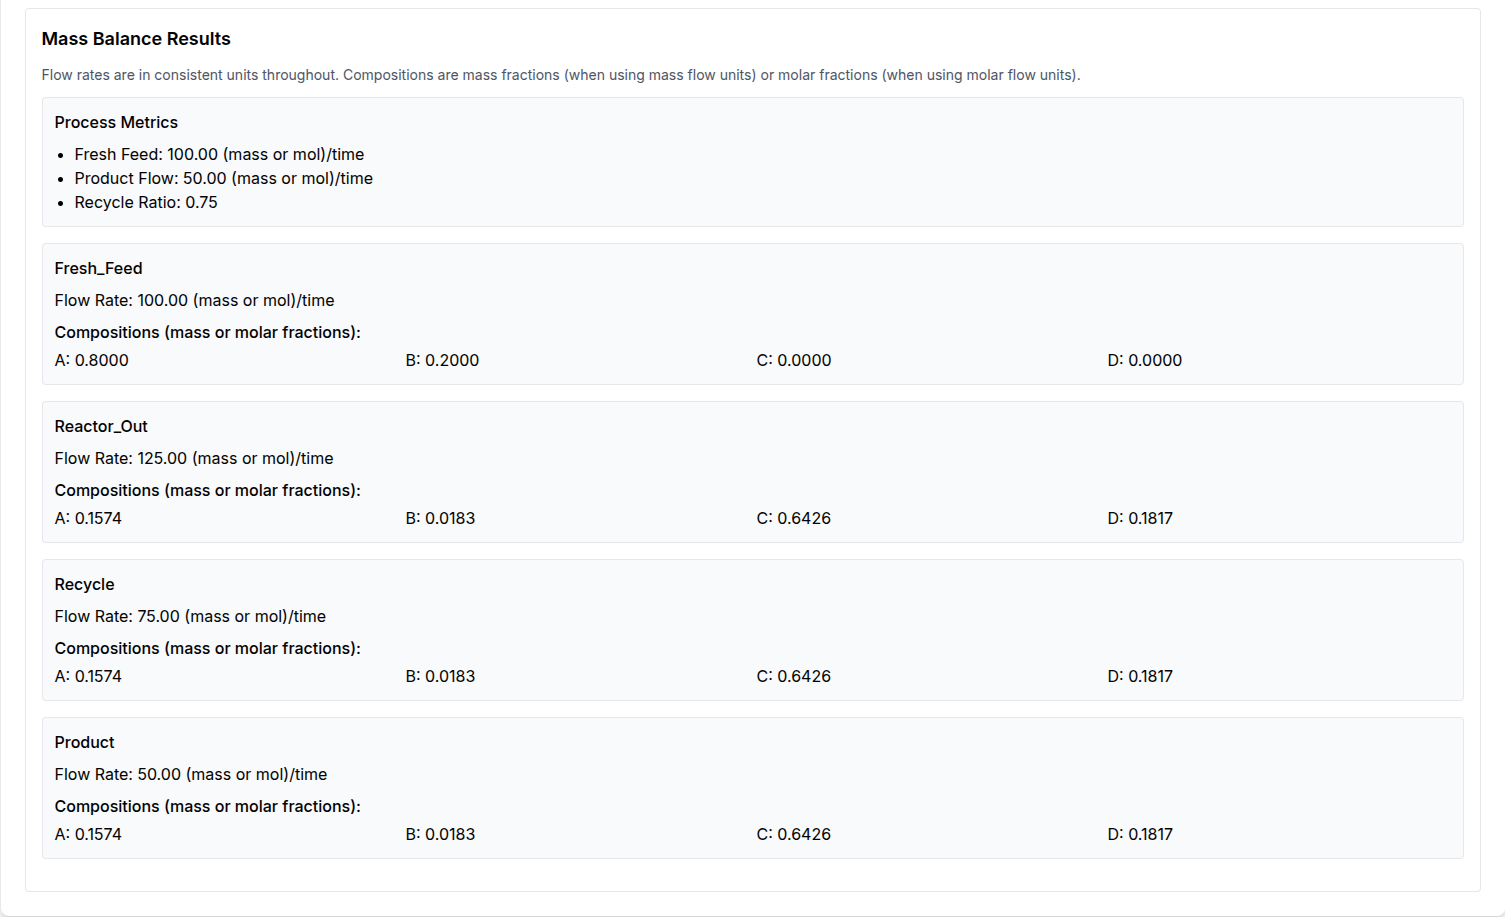
\includegraphics[width=\linewidth]{media/cap4_resultados_balanco_massa_reacao_reciclo.png}
    \fonte{Elaboração própria (2026).}
    \label{fig:mass_balance_results}
\end{figure}

O balanço de massa fundamenta o dimensionamento de equipamentos como misturadores, separadores, reatores e redes de processo, além de embasar análises econômicas (minimizando perdas de matérias-primas) e de segurança (evitando acúmulo indesejado de compostos). Vale notar que temperatura e pressão influenciam o balanço apenas através de propriedades físicas (massa específica, volumes específicos), ou mudanças de fase que afetem as vazões mássicas e molares de cada corrente \cite{felder2005}.

\subsection{Escoamento, Perdas de Carga e Diâmetros Hidráulicos}

O comportamento do escoamento em dutos é governado, principalmente, pelo número de Reynolds, que permite classificar o regime como laminar, de transição ou turbulento. Variáveis-chave incluem o diâmetro hidráulico, a velocidade média, a viscosidade e a massa específica do fluido, bem como a rugosidade relativa da parede. Perfis de velocidade, mecanismos de mistura e dissipação de energia por atrito dependem desse regime de escoamento. Para quantificar a perda de carga (queda de pressão) devida ao atrito no escoamento, emprega-se a equação universal de Darcy–Weisbach \cite{white2018}.

No regime turbulento, o fator de atrito $f$ depende de $Re$ e da rugosidade relativa $\varepsilon/D$, não possuindo solução analítica explícita; por isso, utilizam-se relações empíricas ou aproximadas. Já no regime laminar ($Re < 2300$), o perfil de velocidades é parabólico e $f$ admite a expressão simples dada pela Equação \ref{eq:laminar_friction}:
\begin{equation}
f = \frac{64}{Re}
\label{eq:laminar_friction}
\end{equation}.

Em serviços de água a escoamento turbulento, a fórmula empírica de Hazen--Williams é comumente empregada como aproximação prática \cite{perry2007}. Temperatura e pressão afetam massa específica e viscosidade do fluido, modificando o valor de $Re$ e, consequentemente, as perdas de carga.

Além disso, o material e condições da tubulação (nova, envelhecida) determinam a rugosidade efetiva. Todos esses efeitos impactam diretamente o balanço de energia no escoamento em dutos e a potência requerida em bombas ou compressores \cite{perry2007,white2018}.

\subsubsection{Número de Reynolds}

O número de Reynolds ($Re$) é adimensional e relaciona as forças inerciais com as forças viscosas no escoamento dentro de um duto:

Usando viscosidade dinâmica $\mu$: 
\begin{equation}
Re = \frac{D \cdot V \cdot \rho}{\mu} 
\label{eq:reynolds_din}
\end{equation}

Usando viscosidade cinemática $\nu$: 
\begin{equation}
Re = \frac{D \cdot V}{\nu}
\label{eq:reynolds_cin}
\end{equation}

Onde $D$ é o diâmetro hidráulico, $\rho$ é a massa específica do fluido, $V$ é a velocidade média e $\mu$ é a viscosidade dinâmica. Tipicamente, $Re < 2300$ indica regime laminar, $2300 < Re < 4000$ indica regime de transição, e $Re > 4000$ indica regime turbulento plenamente desenvolvido \cite{white2018}.

\begin{figure}[H]
    \centering
    \caption{Cálculo do Reynolds – Parte 1/3}
    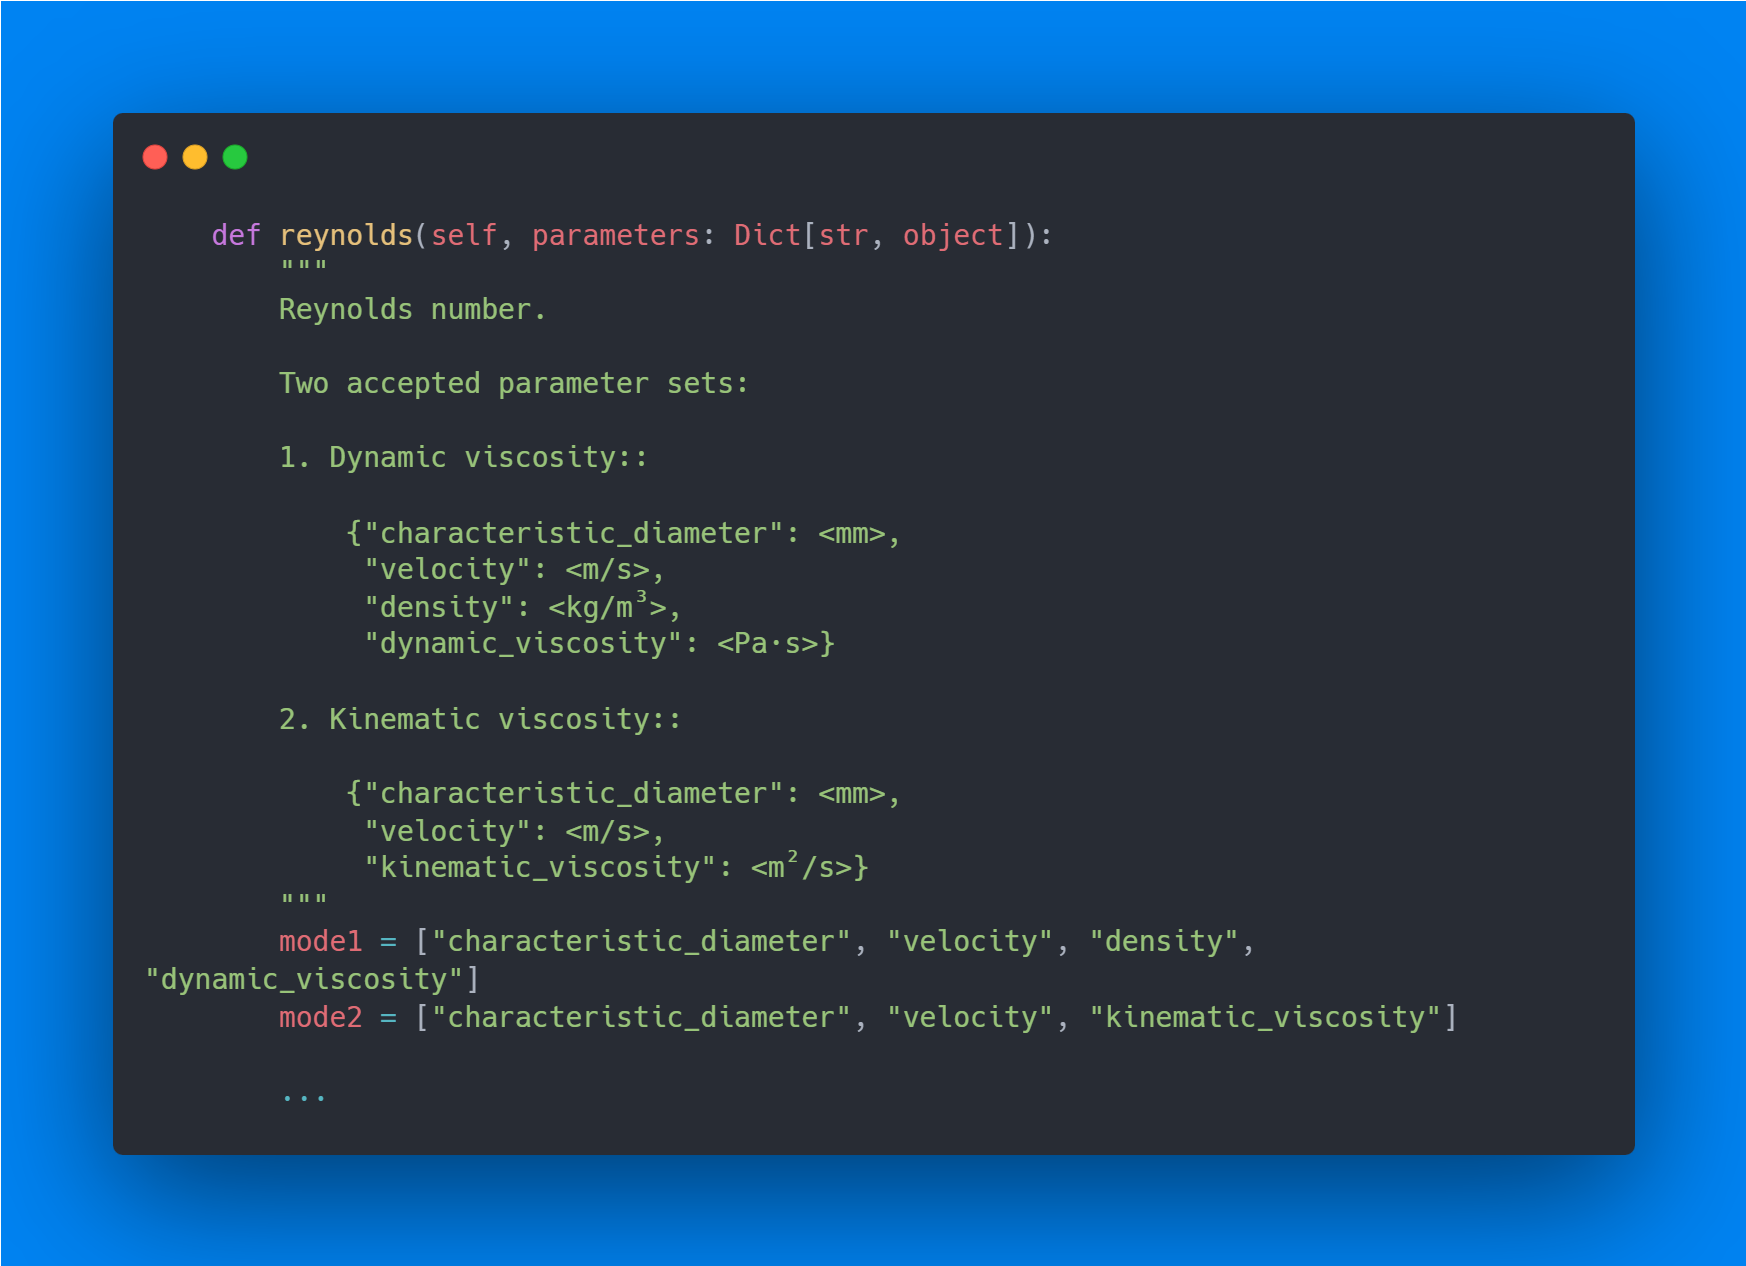
\includegraphics[width=\linewidth]{media/cap4_reynolds_parte_um.png}
    \fonte{Elaboração própria (2026).}
\end{figure}

\begin{figure}[H]
    \centering
    \caption{Cálculo do Reynolds – Parte 2/3}
    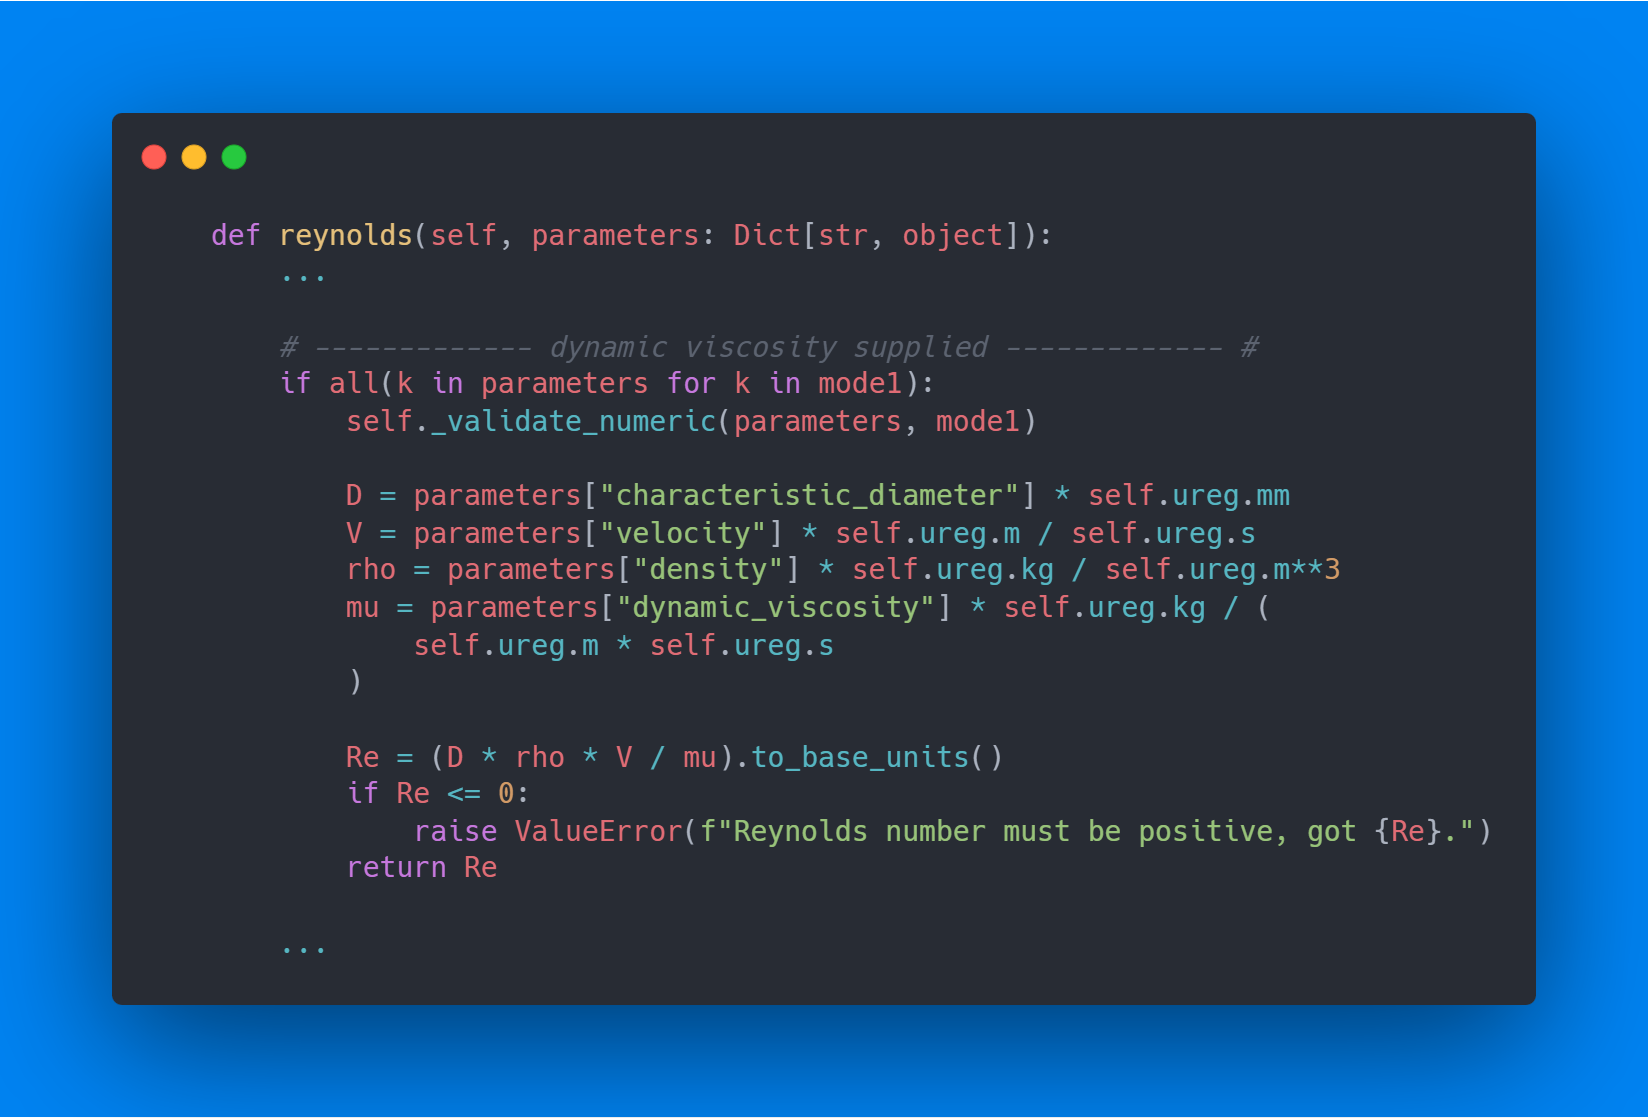
\includegraphics[width=\linewidth]{media/cap4_reynolds_parte_dois.png}
    \fonte{Elaboração própria (2026).}
\end{figure}

\begin{figure}[H]
    \centering
    \caption{Cálculo do Reynolds – Parte 3/3}
    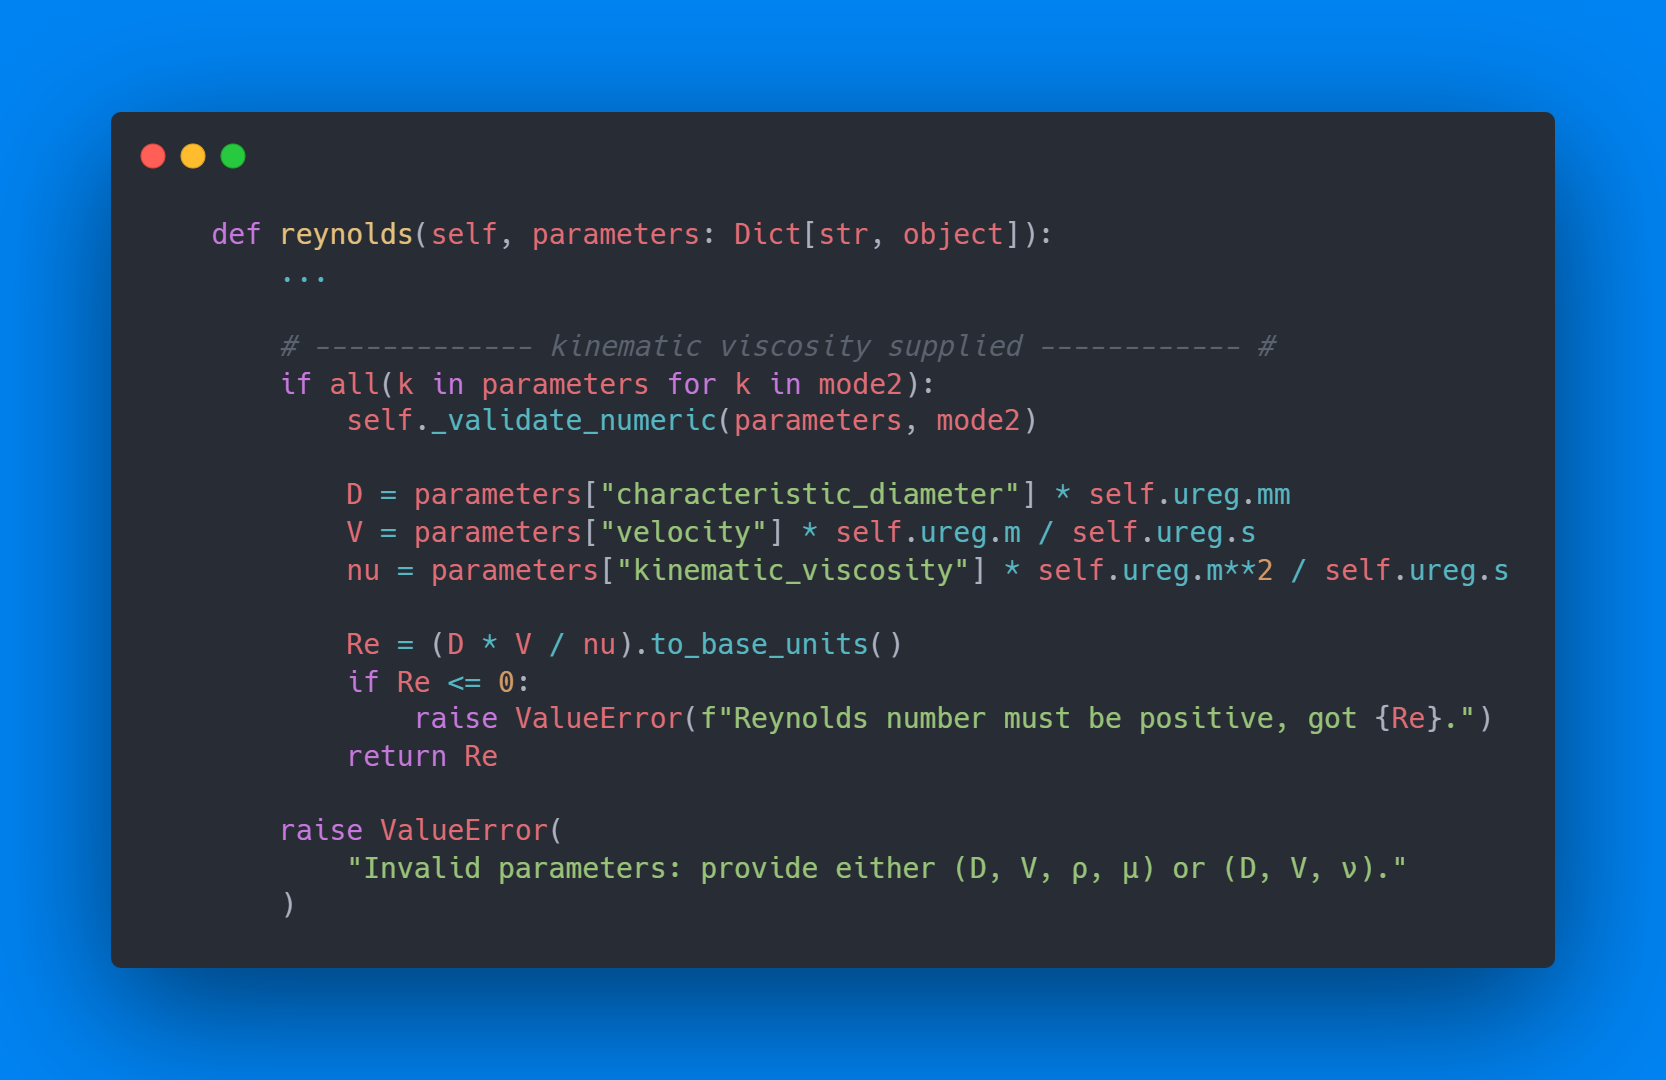
\includegraphics[width=\linewidth]{media/cap4_reynolds_parte_tres.png}
    \fonte{Elaboração própria (2026).}
\end{figure}

\subsubsection{Fator de Atrito}

No regime laminar, o fator de atrito de Darcy pode ser obtido diretamente por $f = 64/Re$. No regime turbulento, $f$ satisfaz implicitamente a equação de Colebrook--White \cite{colebrook1939}:

\begin{equation}
\frac{1}{\sqrt{f}} = -2 \log_{10} \left( \frac{\varepsilon}{3{,}7D_{h}} + \frac{2{,}51}{Re\sqrt{f}} \right)
\label{eq:colebrook}
\end{equation}

Sendo $\varepsilon$ a rugosidade absoluta. Para evitar a resolução iterativa, existem correlações explícitas aproximadas amplamente usadas, por exemplo:

Swamee--Jain \cite{swamee1976}:

\begin{equation}
f = \frac{0{,}25}{\left[\log_{10}\left( \frac{\varepsilon}{3{,}7D} + \frac{5{,}74}{Re^{0{,}9}} \right)\right]^2}
\label{eq:swamee}
\end{equation}

Haaland \cite{haaland1983}:

\begin{equation}
\frac{1}{\sqrt{f}} = -1{,}8 \log_{10} \left[ \left(\frac{\varepsilon/D}{3{,}7}\right)^{1{,}11} + \frac{6{,}9}{Re} \right]
\label{eq:haaland}
\end{equation}

O \textit{software} implementa as equações acima para cálculo de $f$ conforme o regime e dados disponíveis \cite{white2018}. A interface para a obtenção do fator de atrito e as opções disponibilizadas ao usuário estão exibidas na Figura \ref{fig:friction_factor_calc}.

\begin{figure}[H]
    \centering
    \caption{Interface de cálculo do fator de atrito}
    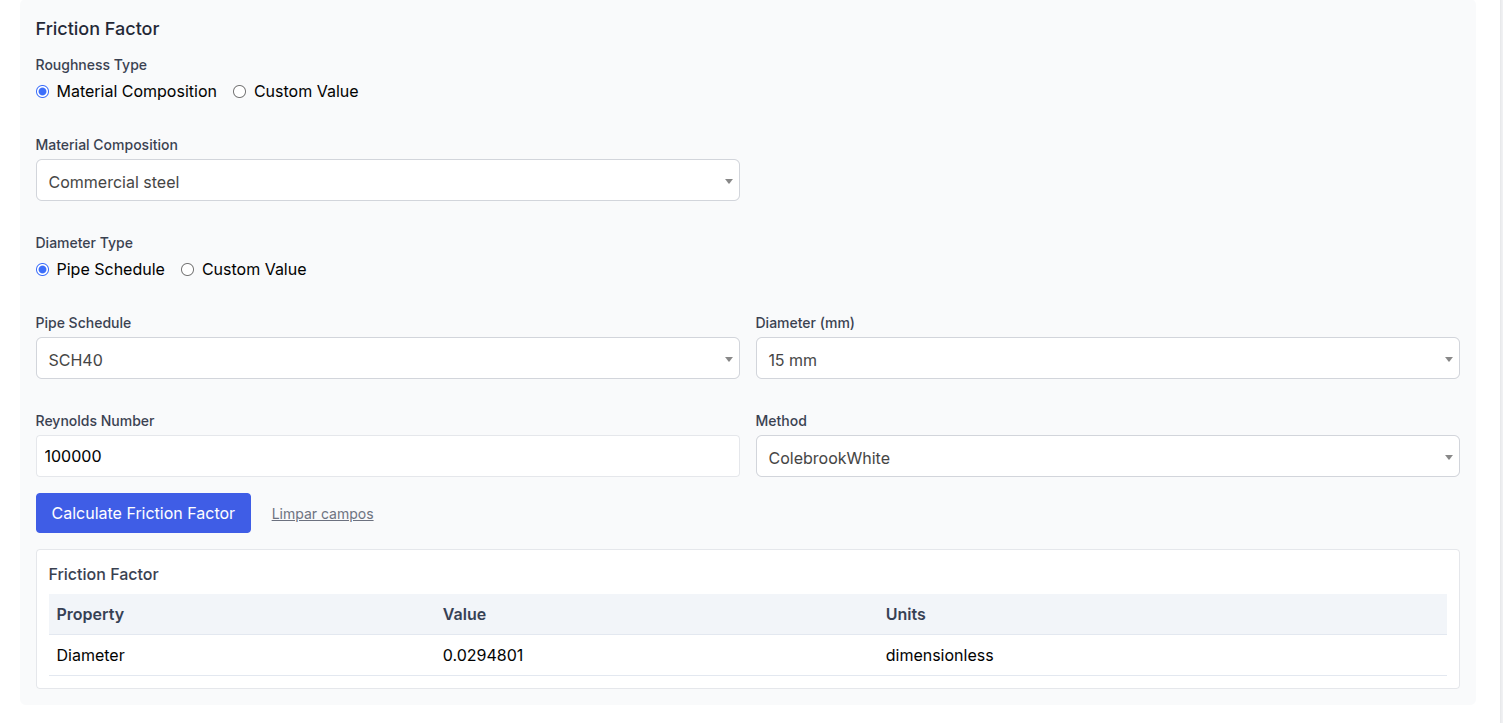
\includegraphics[width=\linewidth]{media/cap4_diagrama_moody.png}
    \fonte{Elaboração própria (2026).}
    \label{fig:friction_factor_calc}
\end{figure}

\begin{figure}[H]
    \centering
    \caption{Cálculo do fator de atrito – Parte 1/2}
    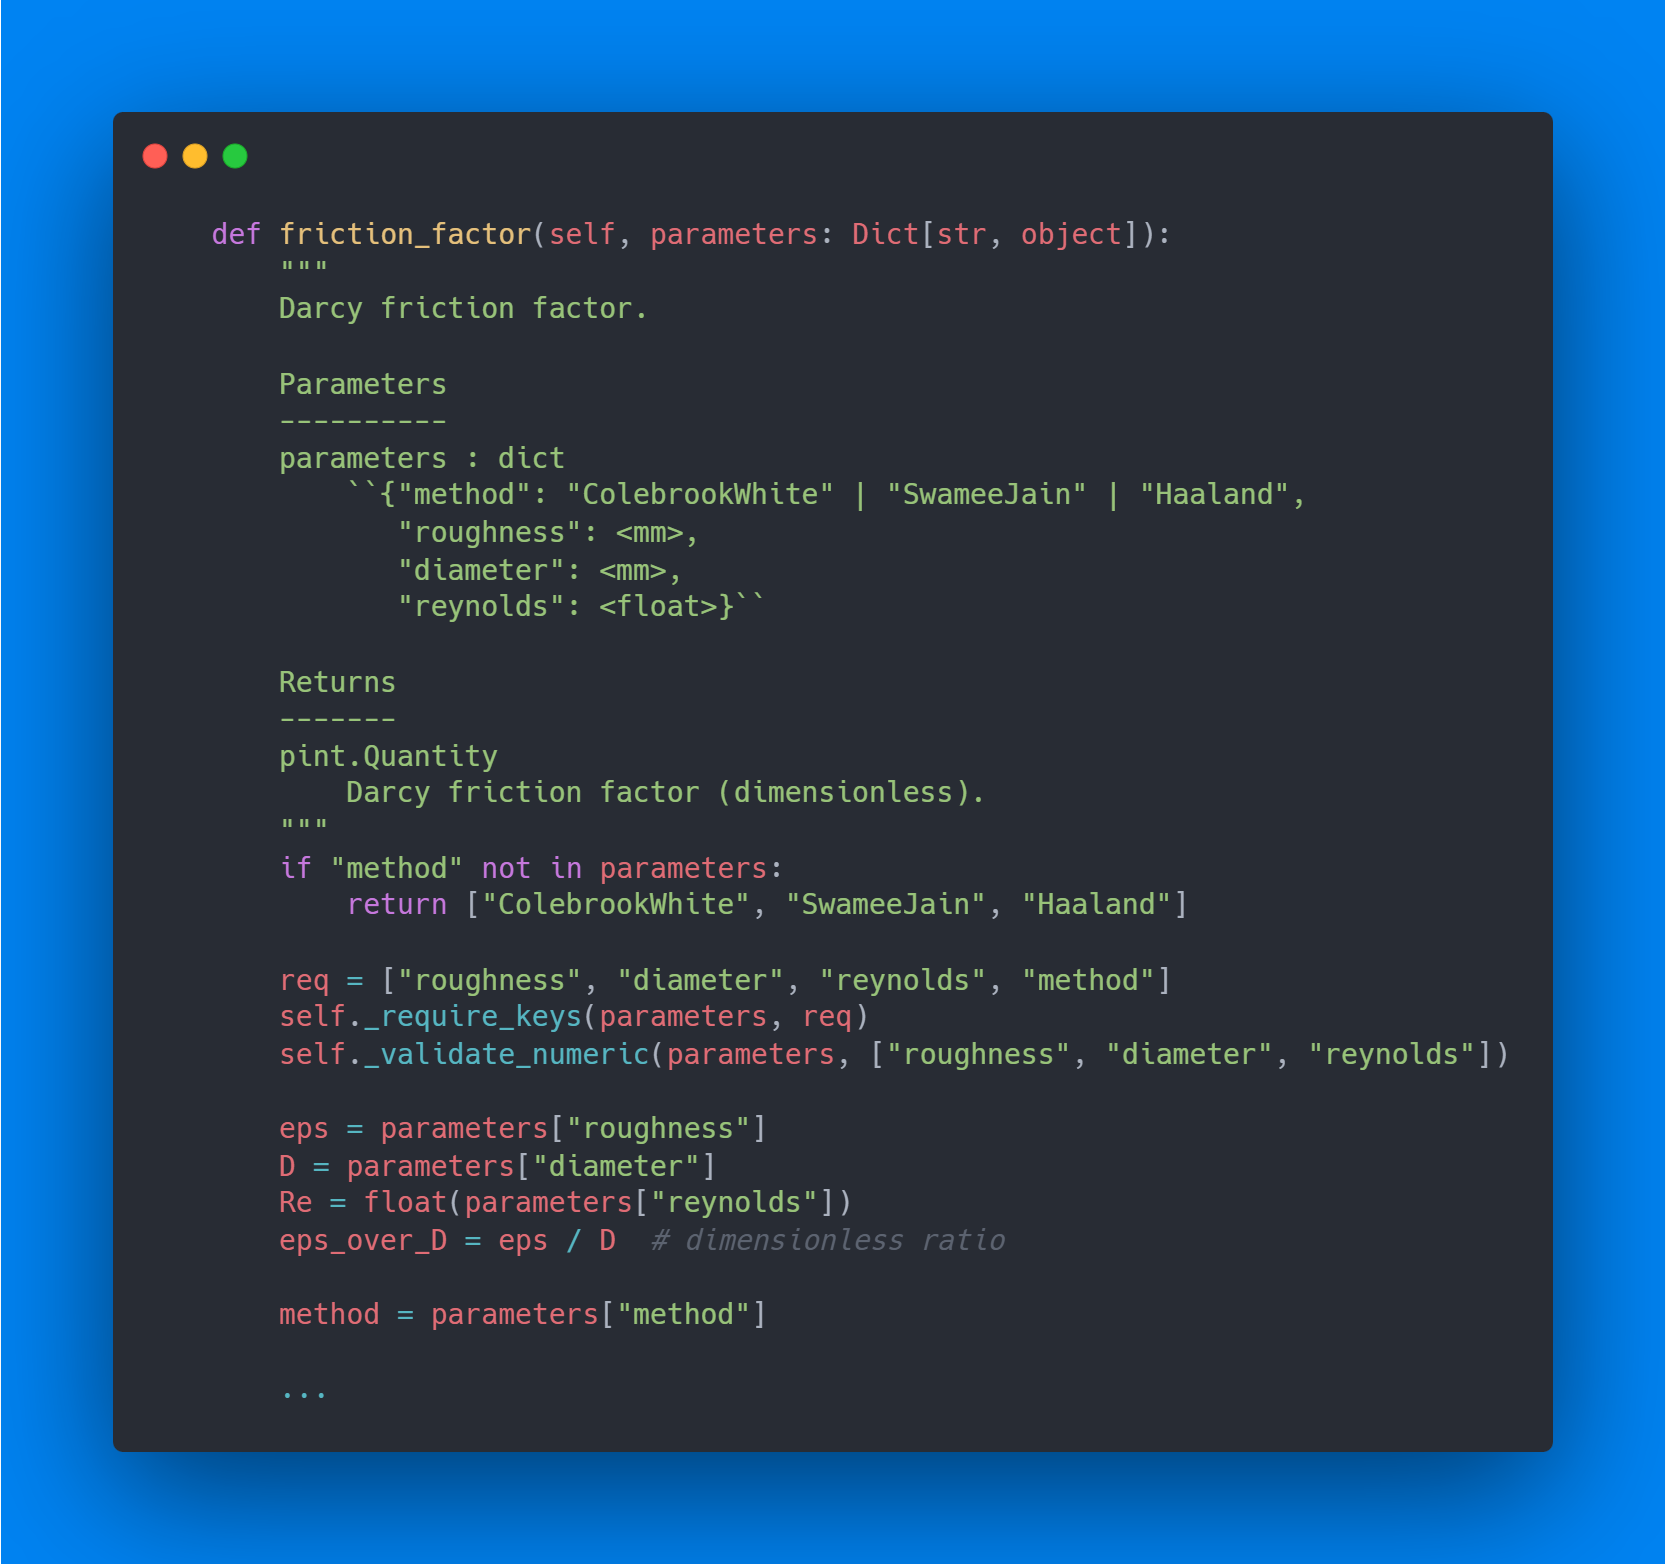
\includegraphics[width=\linewidth]{media/cap4_fator_atrito_parte_um.png}
    \fonte{Elaboração própria (2026).}
\end{figure}

\begin{figure}[H]
    \centering
    \caption{Cálculo do fator de atrito – Parte 2/2}
    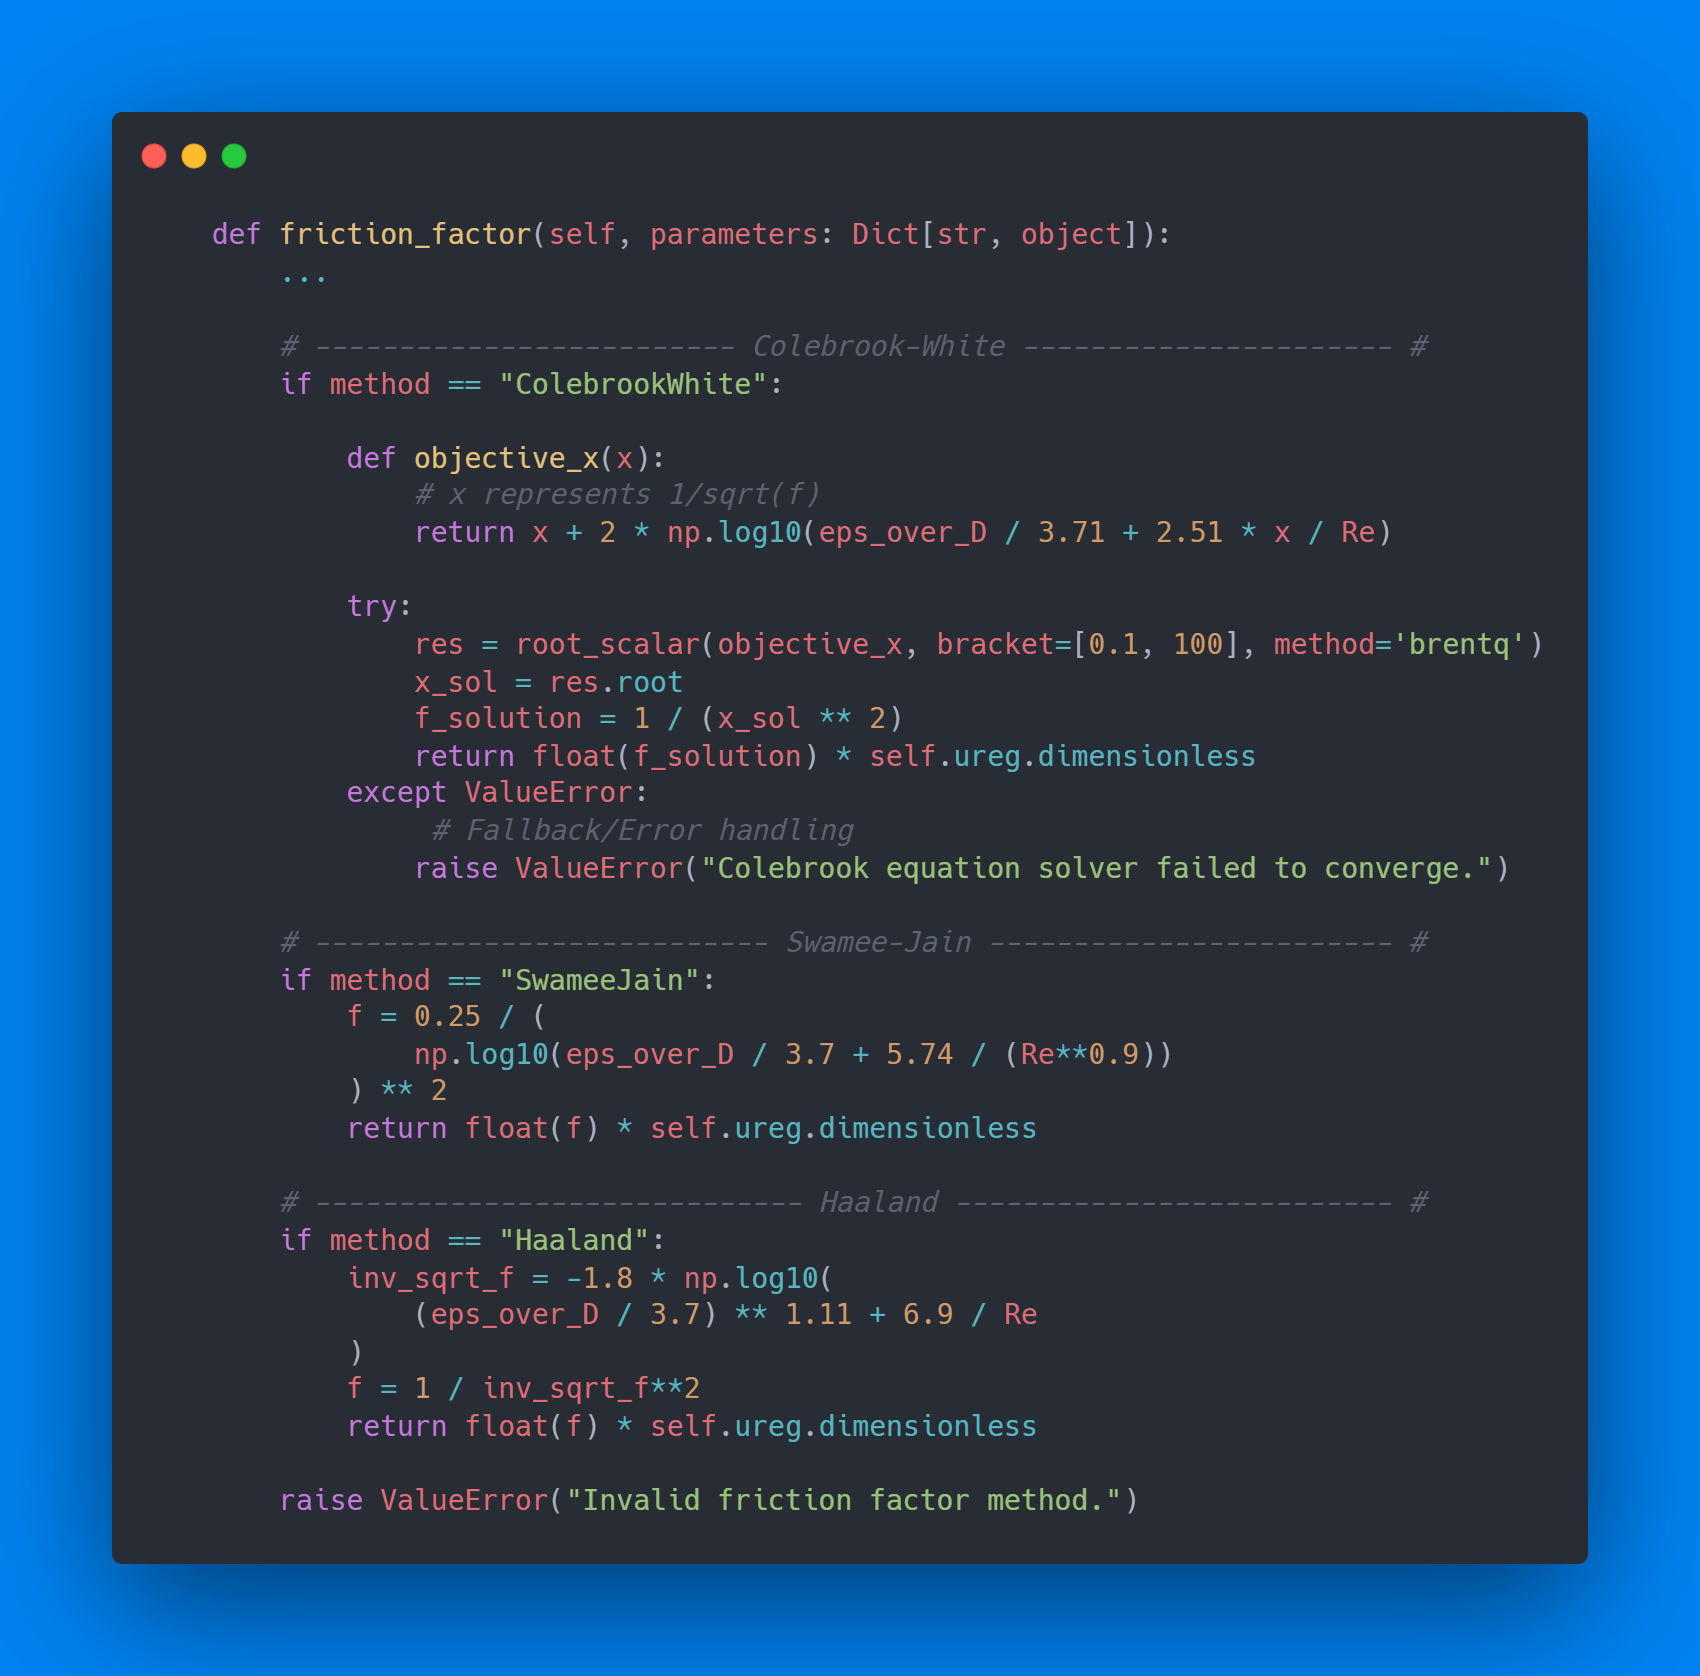
\includegraphics[width=\linewidth]{media/cap4_fator_atrito_parte_dois.png}
    \fonte{Elaboração própria (2026).}
\end{figure}

\subsubsection{Perda de Carga -- Darcy--Weisbach e Hazen--Williams}

A perda de carga distribuída $h_{f}$ em uma tubulação de comprimento $L$ é calculada pela equação de Darcy–Weisbach:

\begin{equation}
h_{f} = f \cdot \frac{\left( L + \sum_{}^{} L_{e q} \right)}{D} \frac{V^{2}}{2 g}
\label{eq:darcy}
\end{equation}

Em que $\sum_{}^{} L_{eq}$ é o comprimento equivalente total dos acessórios, em unidades de comprimento, e $g$ é a aceleração da gravidade. Essa fórmula é universal e independe do fluido, desde que $f$ seja adequadamente determinado \cite{perry2007}.

Para escoamento de água em tubulações de diâmetro moderado (tipicamente $D > 50\ \mathrm{mm}$) e regime turbulento plenamente estabelecido, a fórmula empírica de Hazen--Williams pode ser empregada como simplificação:

\begin{equation}
h_{f} = \frac{4{,}73 L}{C^{1{,}852}D^{4{,}87}} Q^{1{,}852}
\label{eq:hazen}
\end{equation}

Em que $Q$ é a vazão volumétrica e $C$ é o coeficiente de Hazen--Williams do material, adimensional e tabelado para tubulações novas de ferro fundido, aço, PVC etc. Apesar de não possuir fundamentação teórica geral, essa equação fornece boa precisão para água a 20\,°C em tubulações de transporte e é consagrada no projeto de redes de água devido à sua simplicidade \cite{perry2007,white2018}.

\begin{figure}[H]
    \centering
    \caption{Cálculo da perda de carga – Parte 1/3}
    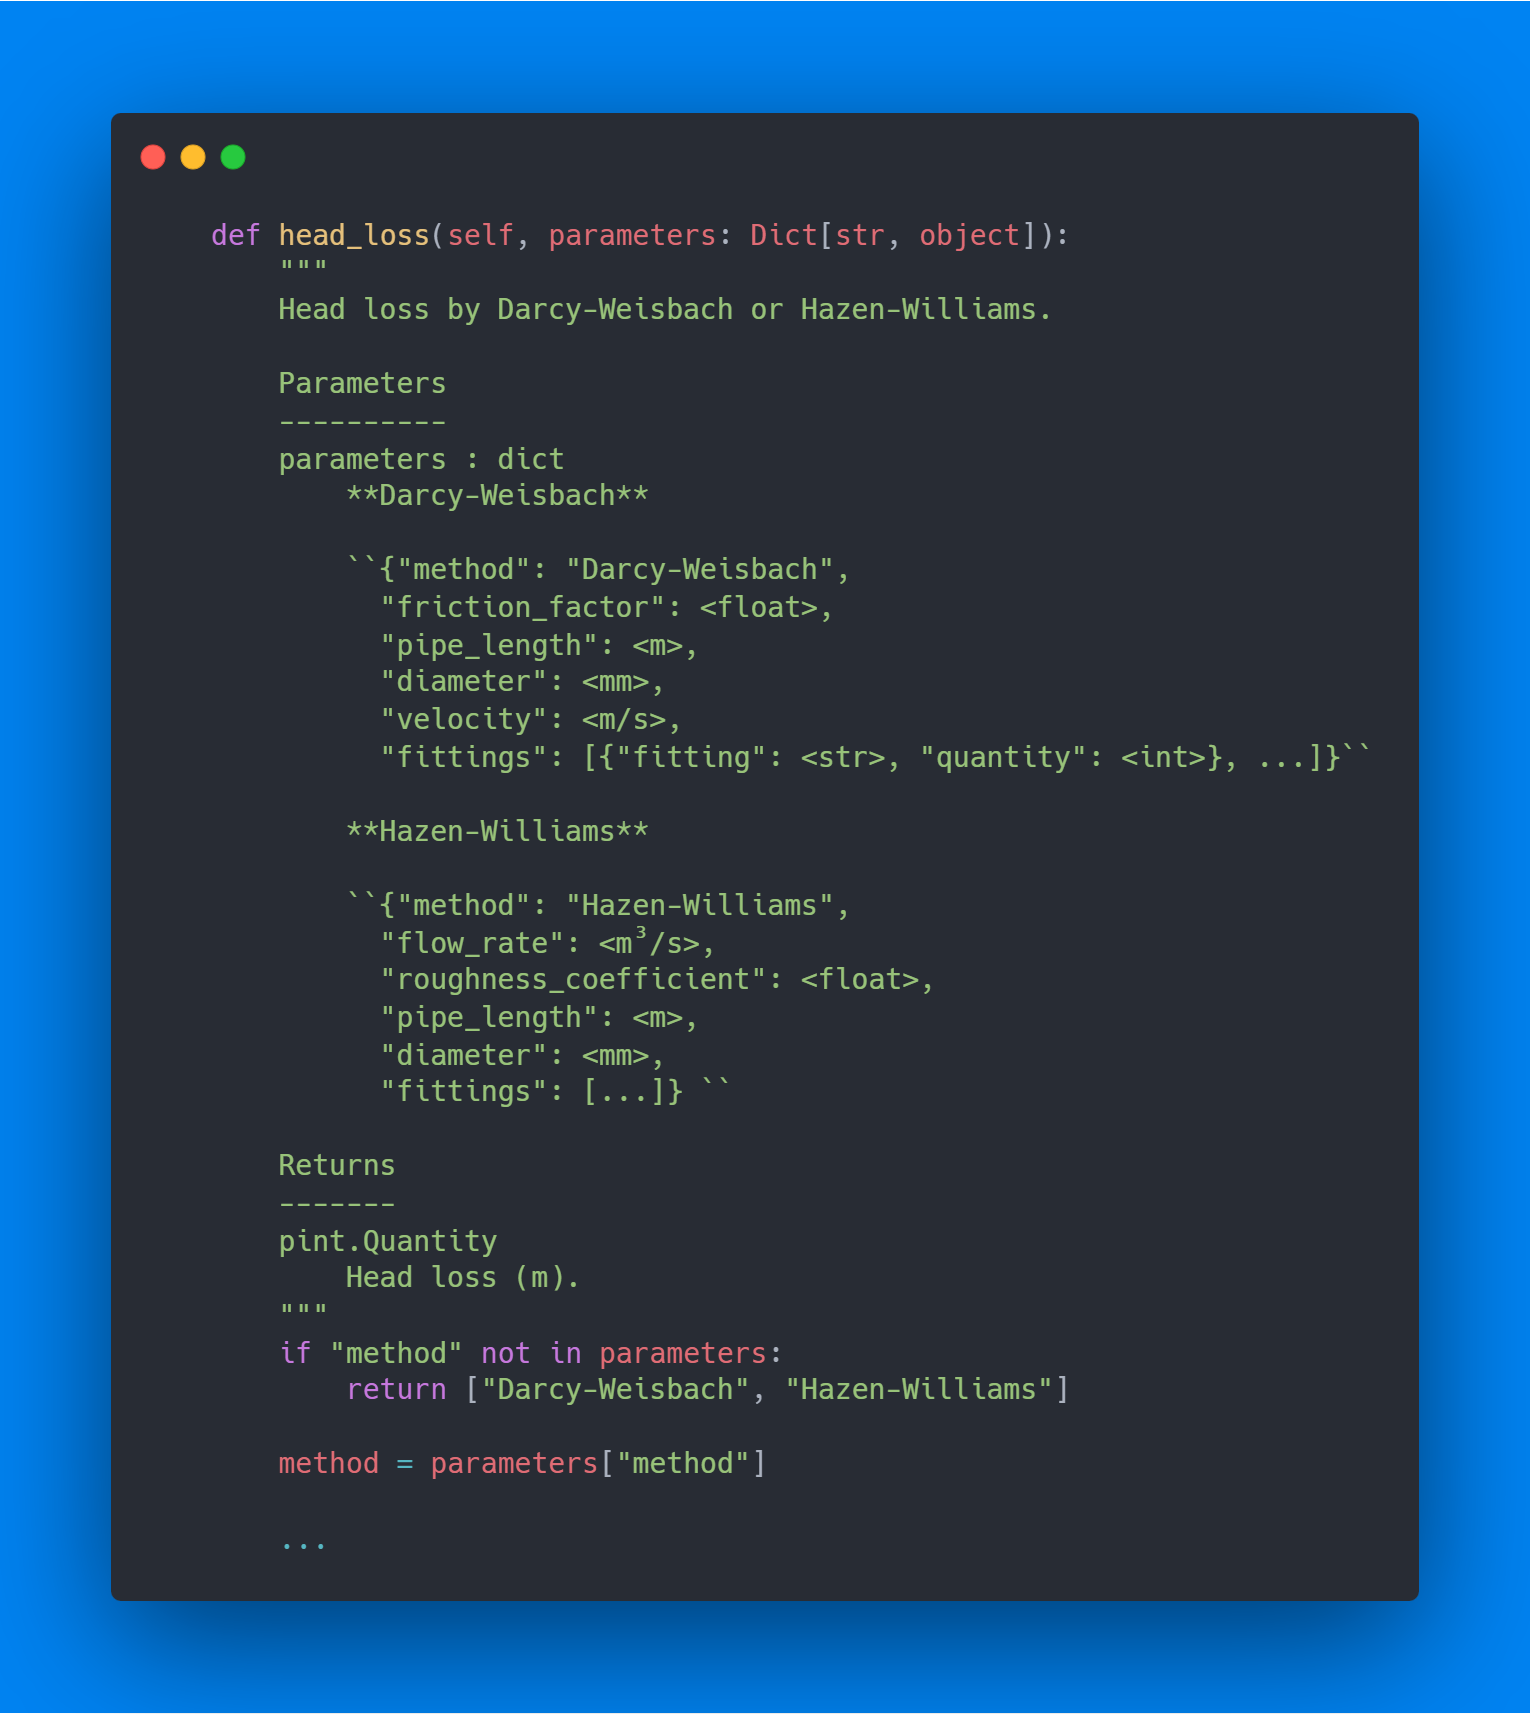
\includegraphics[width=\linewidth]{media/cap4_perda_carga_parte_um.png}
    \fonte{Elaboração própria (2026).}
\end{figure}

\begin{figure}[H]
    \centering
    \caption{Cálculo da perda de carga – Parte 2/3}
    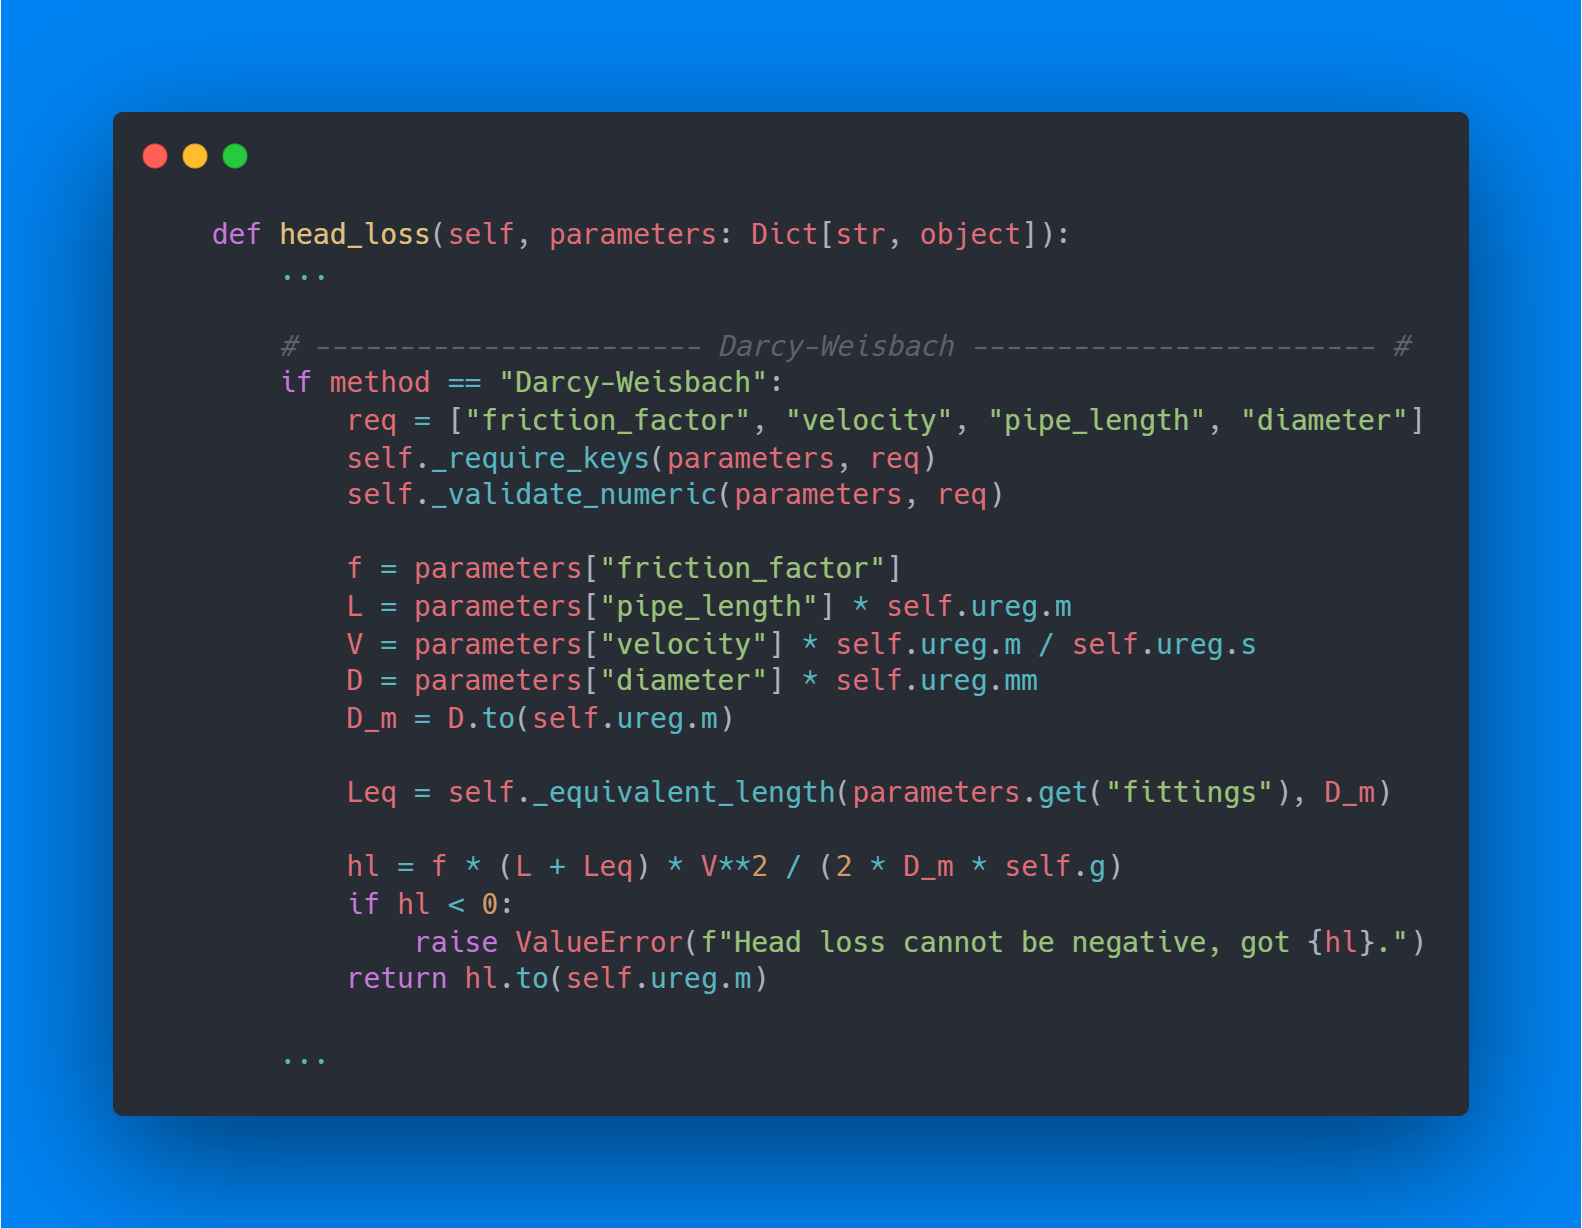
\includegraphics[width=\linewidth]{media/cap4_perda_carga_parte_dois.png}
    \fonte{Elaboração própria (2026).}
\end{figure}

\begin{figure}[H]
    \centering
    \caption{Cálculo da perda de carga – Parte 3/3}
    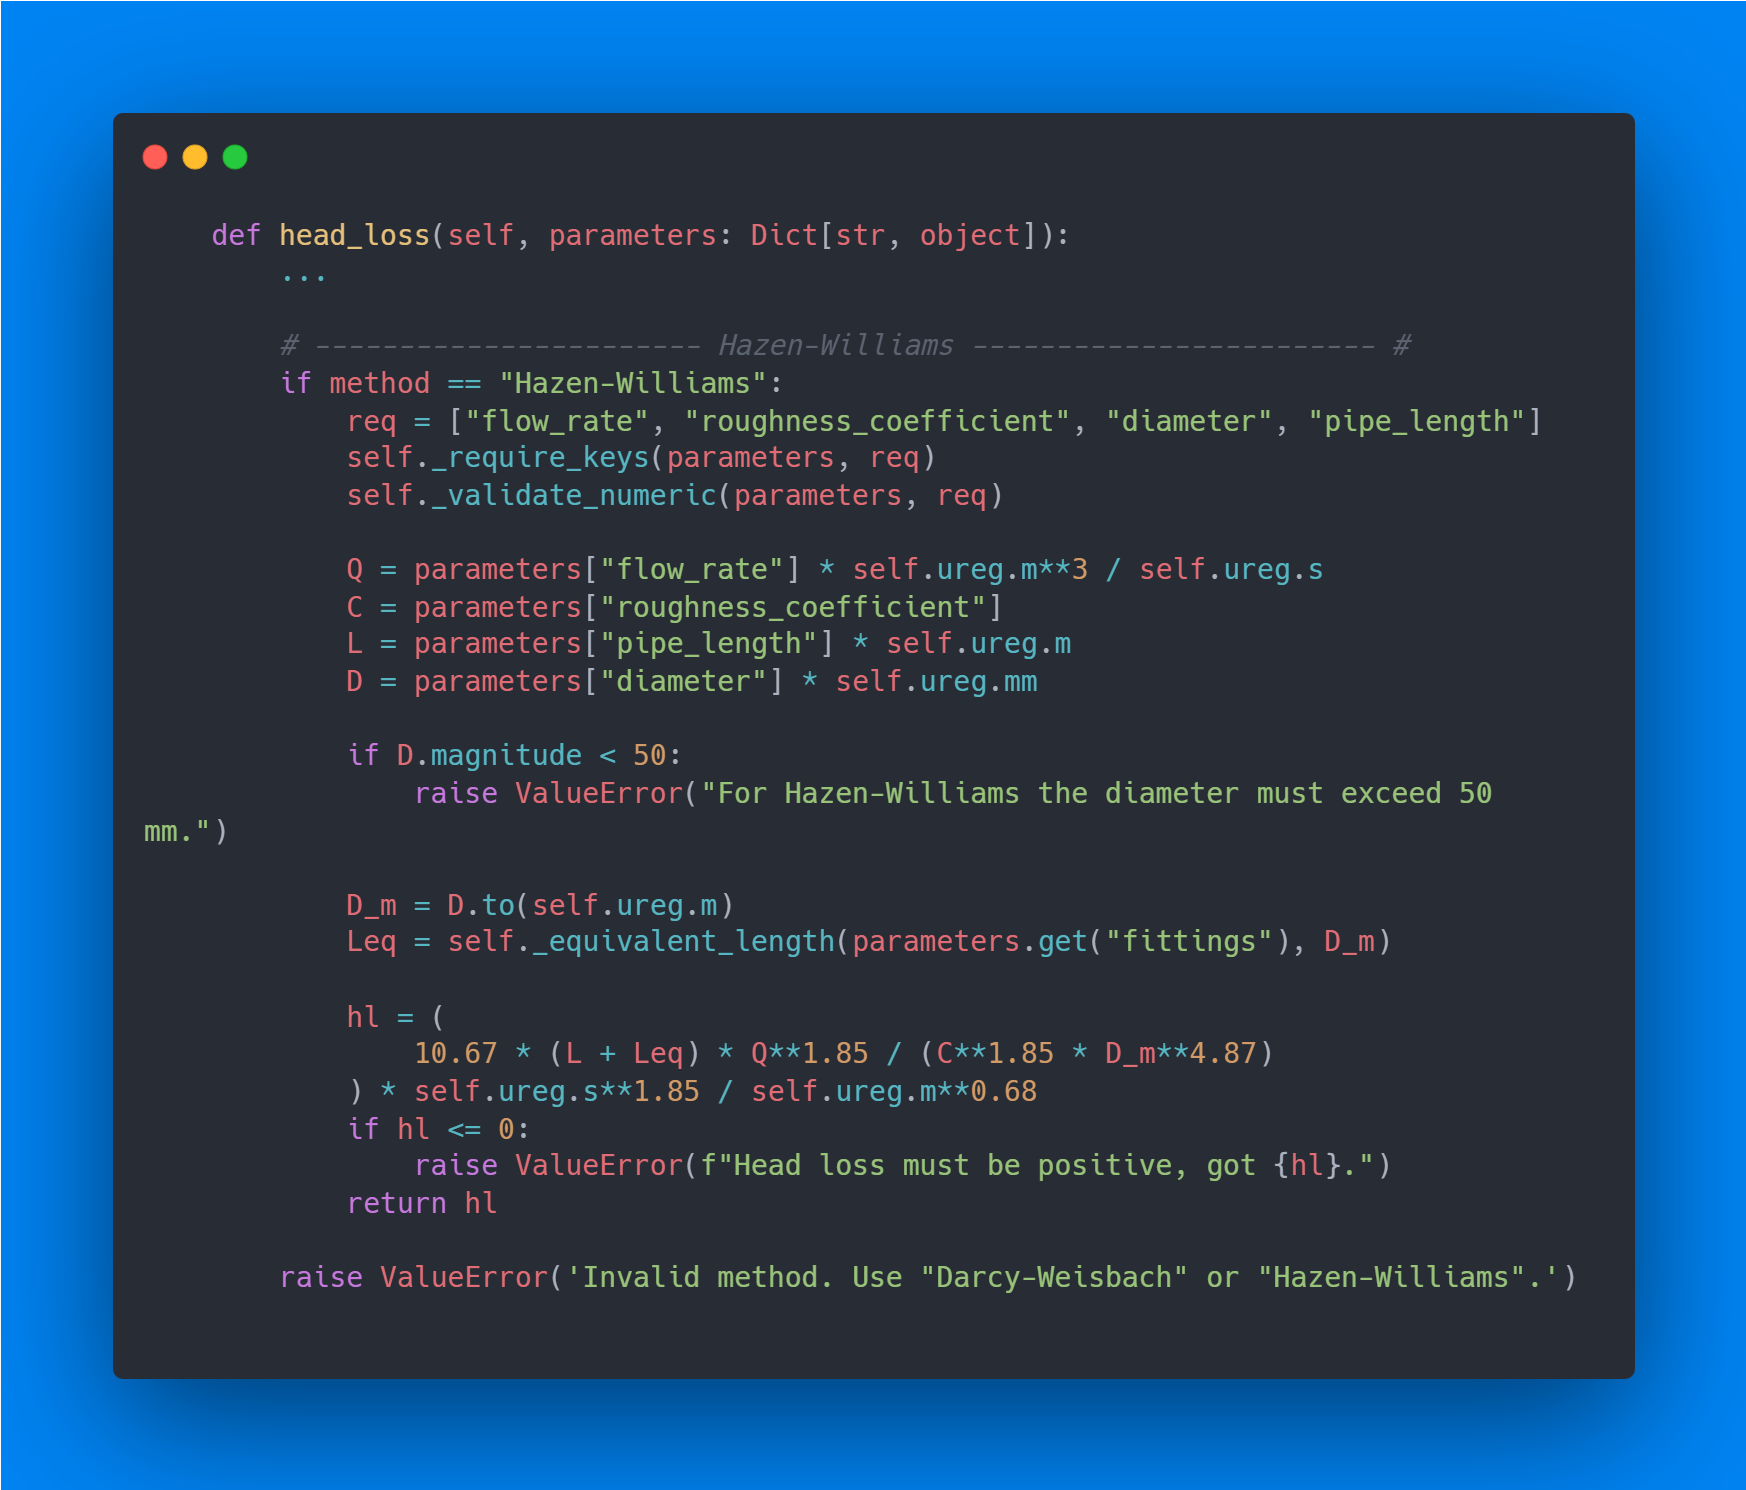
\includegraphics[width=\linewidth]{media/cap4_perda_carga_parte_tres.png}
    \fonte{Elaboração própria (2026).}
\end{figure}

\subsubsection{Altura Manométrica entre Dois Pontos}

A forma estendida da equação de Bernoulli é utilizada para avaliar as variações de carga (energia por unidade de peso do fluido) entre dois pontos de um duto de escoamento, incluindo perdas:

\begin{equation}
H = \frac{P_{2} - P_{1}}{\rho g} + \frac{V_{2}^{2} - V_{1}^{2}}{2 g} + z_{2} - z_{1}
\label{eq:bernoulli}
\end{equation}

Em que $H$ é a altura manométrica adicionada (se positiva) ou removida (se negativa) entre os pontos 1 e 2. Nessa equação, $\frac{P_{2} - P_{1}}{\rho g}$ representa a variação de pressão estática convertida em altura de coluna de fluido, $z_{2} - z_{1}$ é a variação de cota geométrica, o termo de velocidades representa a variação de energia cinética e $h_{f}$ engloba todas as perdas de carga (distribuídas e localizadas) entre os pontos \cite{white2018}.

Essa equação é fundamental para avaliar a necessidade de bombeamento: uma bomba deve fornecer uma $H$ suficiente para superar as perdas e elevar o fluido da condição 1 até 2; inversamente, uma turbomáquina geradora extrairá essa energia do fluido.

\begin{figure}[H]
    \centering
    \caption{Cálculo do \textit{head} – Parte 1/2}
    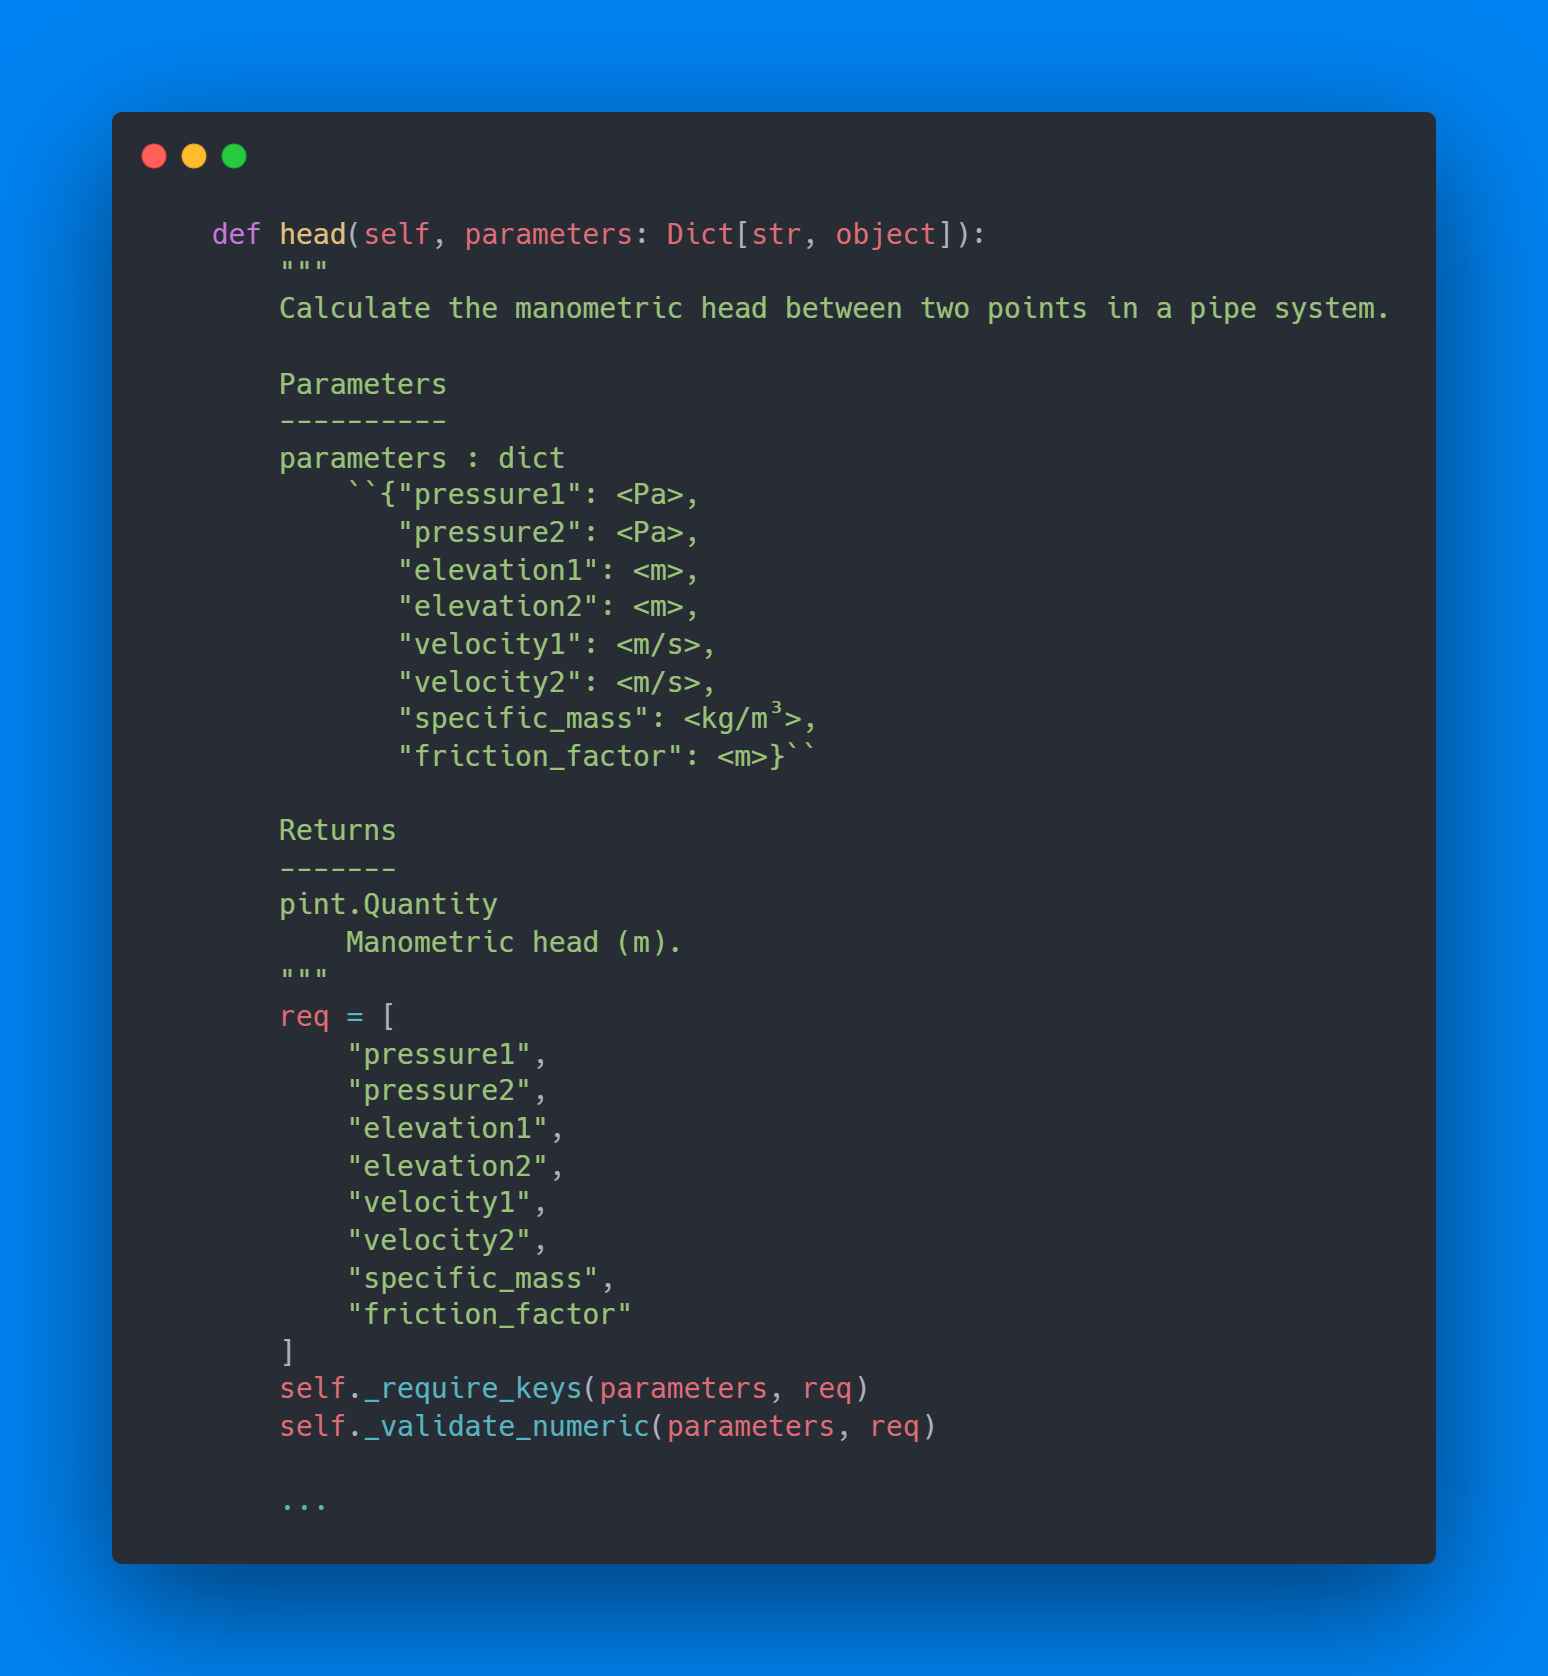
\includegraphics[width=\linewidth]{media/cap4_head_parte_um.png}
    \fonte{Elaboração própria (2026).}
\end{figure}

\begin{figure}[H]
    \centering
    \caption{Cálculo do \textit{head} – Parte 2/2}
    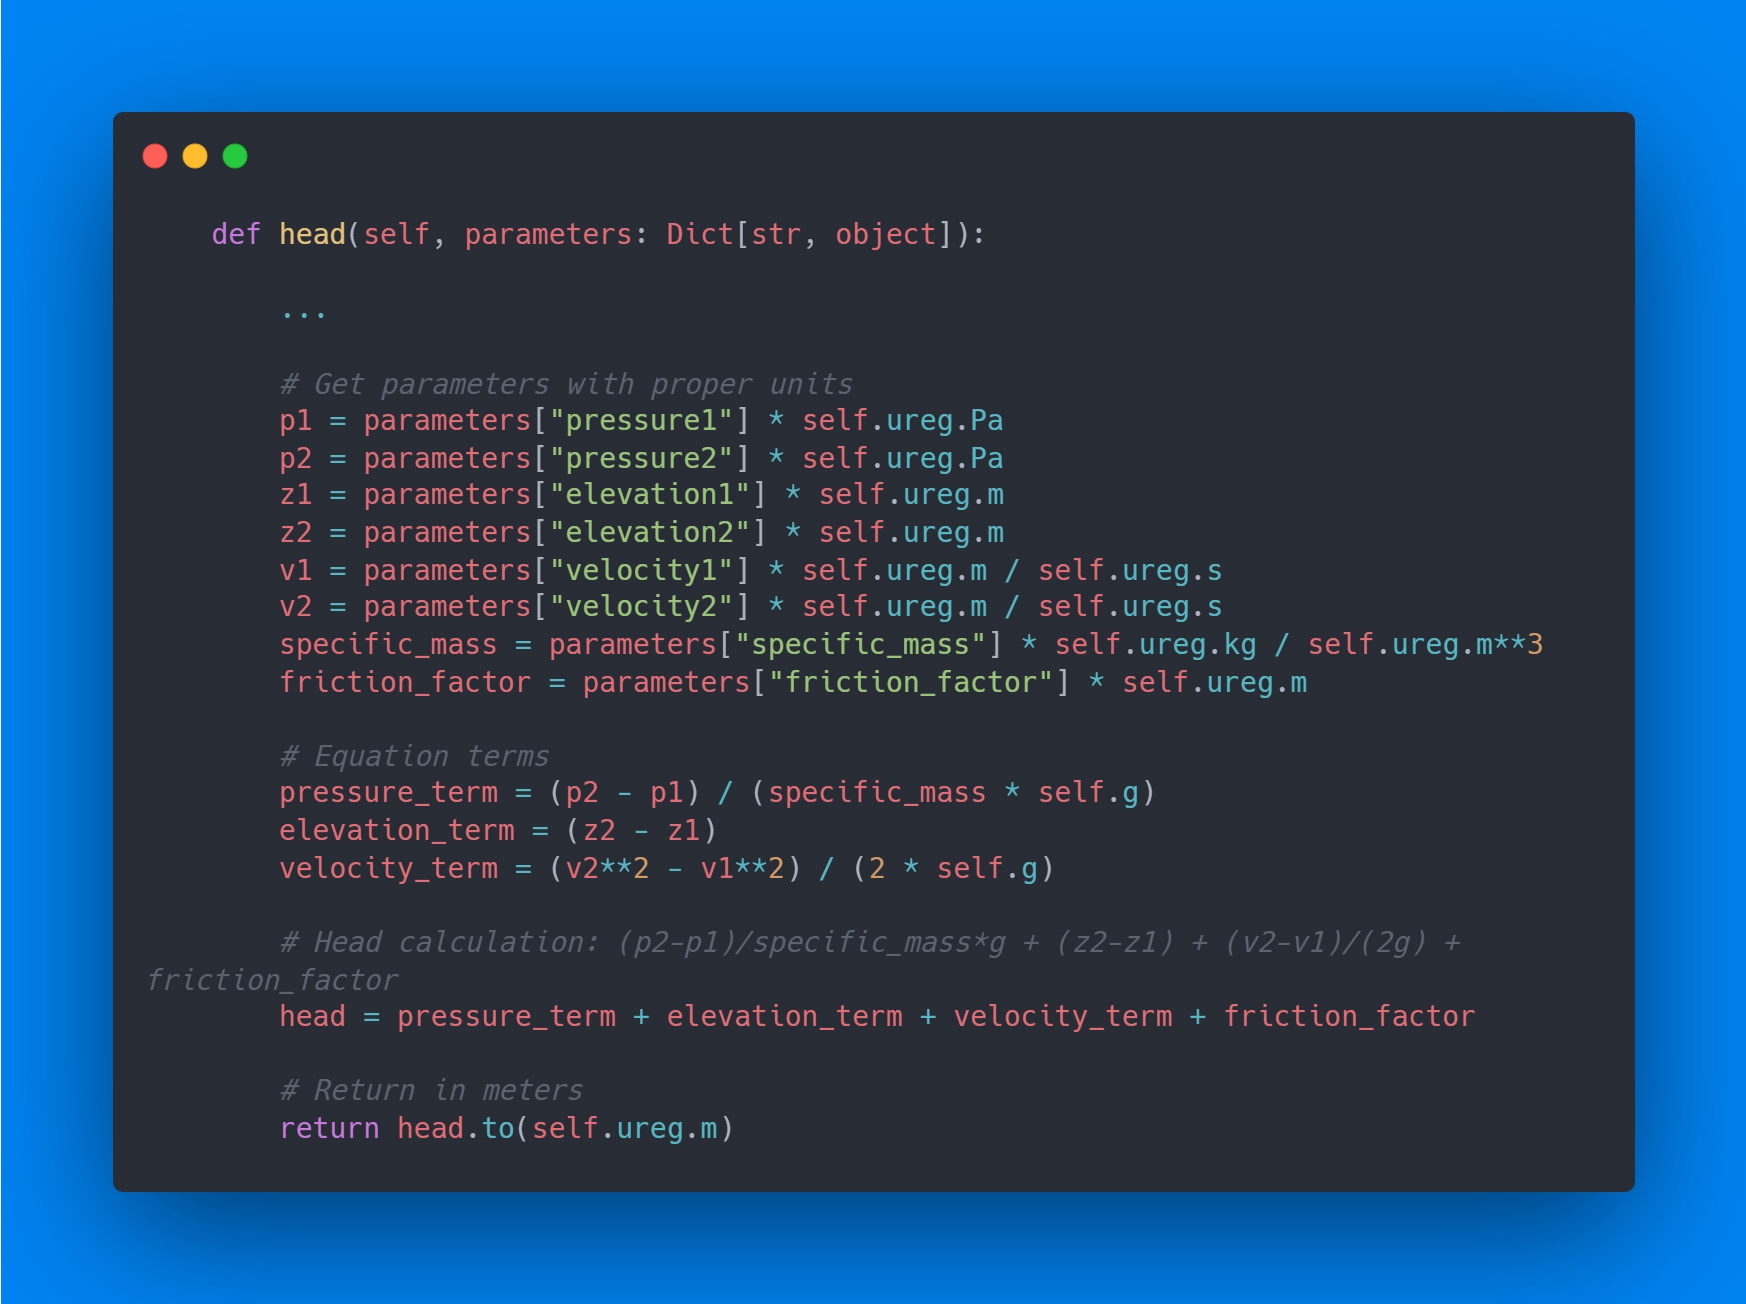
\includegraphics[width=\linewidth]{media/cap4_head_parte_dois.png}
    \fonte{Elaboração própria (2026).}
\end{figure}

\subsubsection{\textit{NPSH} Disponível}

Para evitar cavitação em bombas, calcula-se o \textit{NPSH} disponível na sucção, que deve exceder o \textit{NPSH} requerido pelo fabricante. A expressão para o \textit{NPSH} disponível, em termos de altura de líquido, é:

\begin{equation}
N P S H_{d i s p} = \frac{P_{s u c} + P_{a t m} - p_{v a p}}{\rho g} + \frac{V_{s u c}^{2} \ }{2 g} + \left( z_{s u c} - z_{0} \right) - h_{s u c}
\label{eq:npsh}
\end{equation}

Sendo $P_{suc}$ a pressão manométrica na linha de sucção da bomba, $P_{atm}$ a pressão atmosférica, $z_{suc}$ a elevação do ponto de sucção em relação à referência, $v_{suc}$ a velocidade do fluido na sucção, $h_{suc}$ as perdas de carga na linha de sucção e $p_{vap}$ a pressão de vapor do líquido na temperatura de bombeamento \cite{perry2007}.

O cálculo de \textit{NPSH} disponível permite verificar se há margem de segurança sobre o \textit{NPSH} requerido da bomba (fornecido pelo fabricante para aquela vazão), garantindo que o líquido não vaporize na entrada da bomba – o que causaria cavitação, danos e redução de desempenho.

\begin{figure}[H]
    \centering
    \caption{Cálculo do \textit{NPSH} – Parte 1/2}
    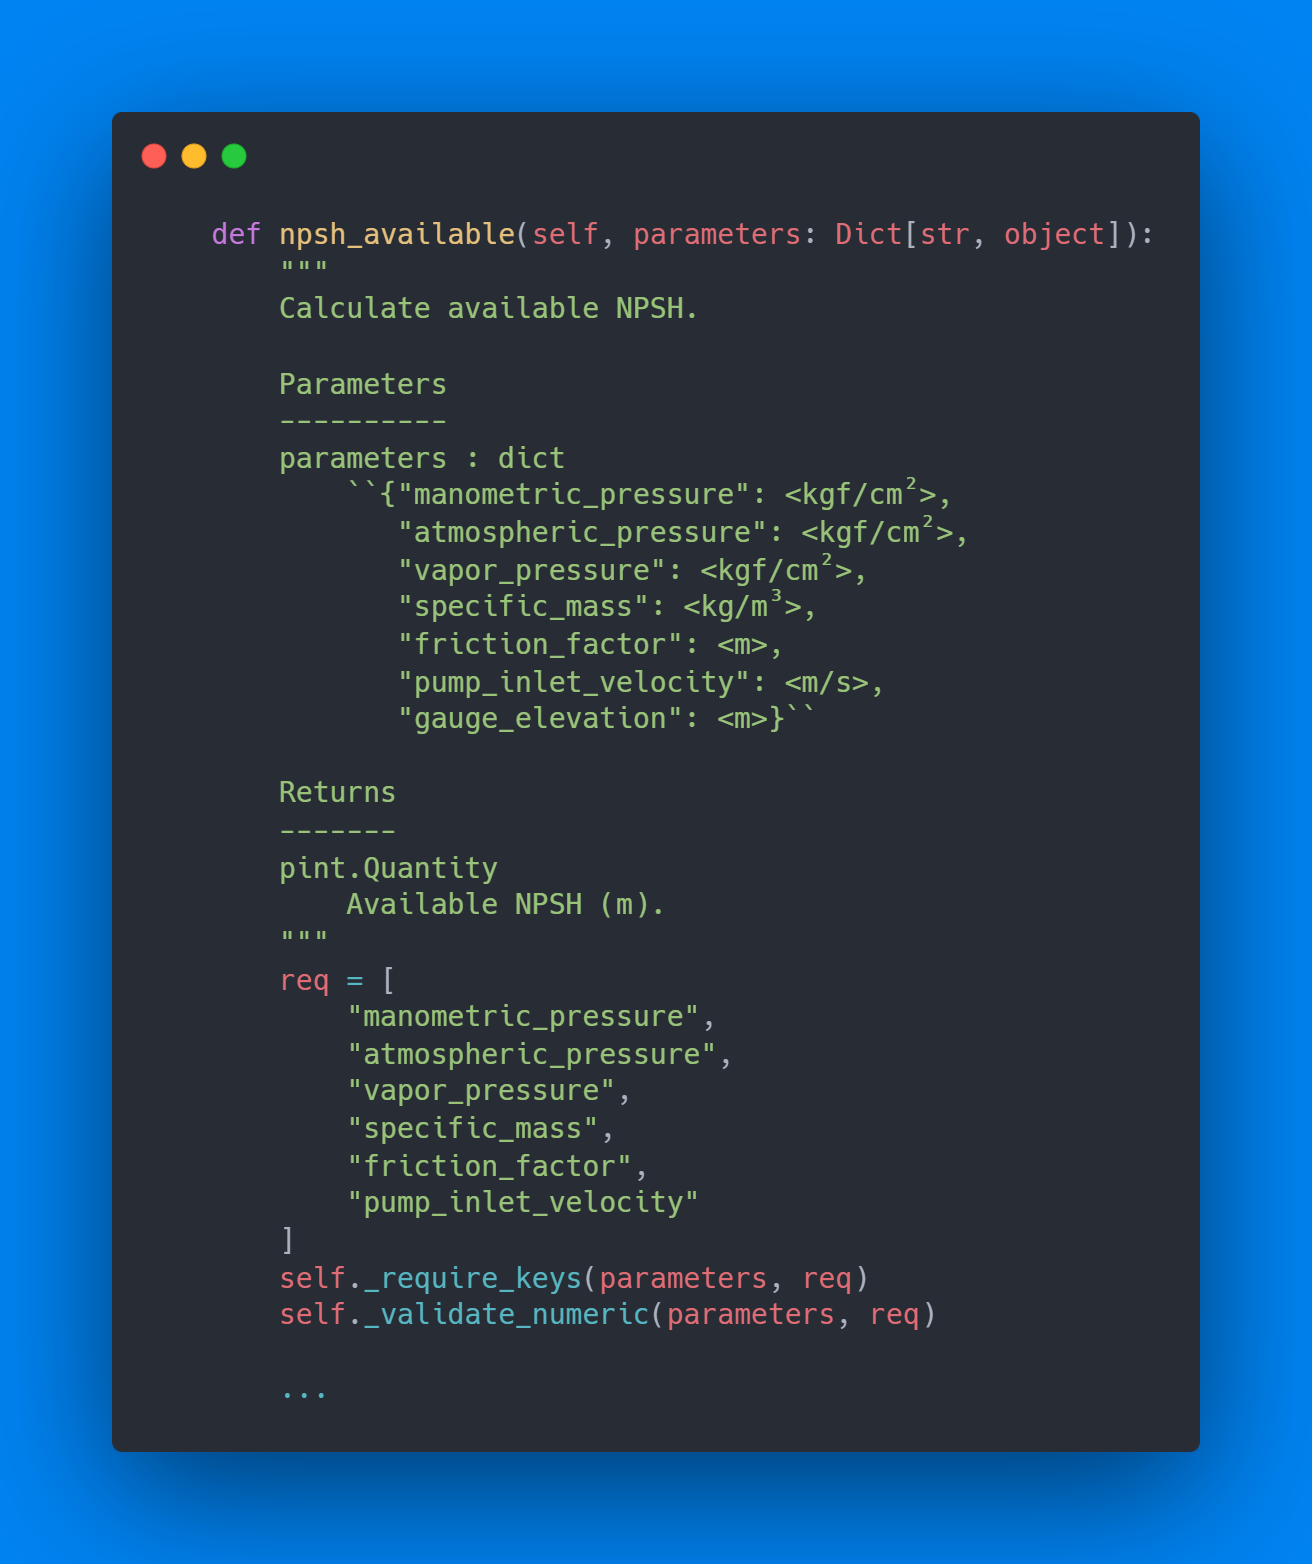
\includegraphics[width=\linewidth]{media/cap4_npsh_parte_um.png}
    \fonte{Elaboração própria (2026).}
\end{figure}

\begin{figure}[H]
    \centering
    \caption{Cálculo do \textit{NPSH} – Parte 2/2}
    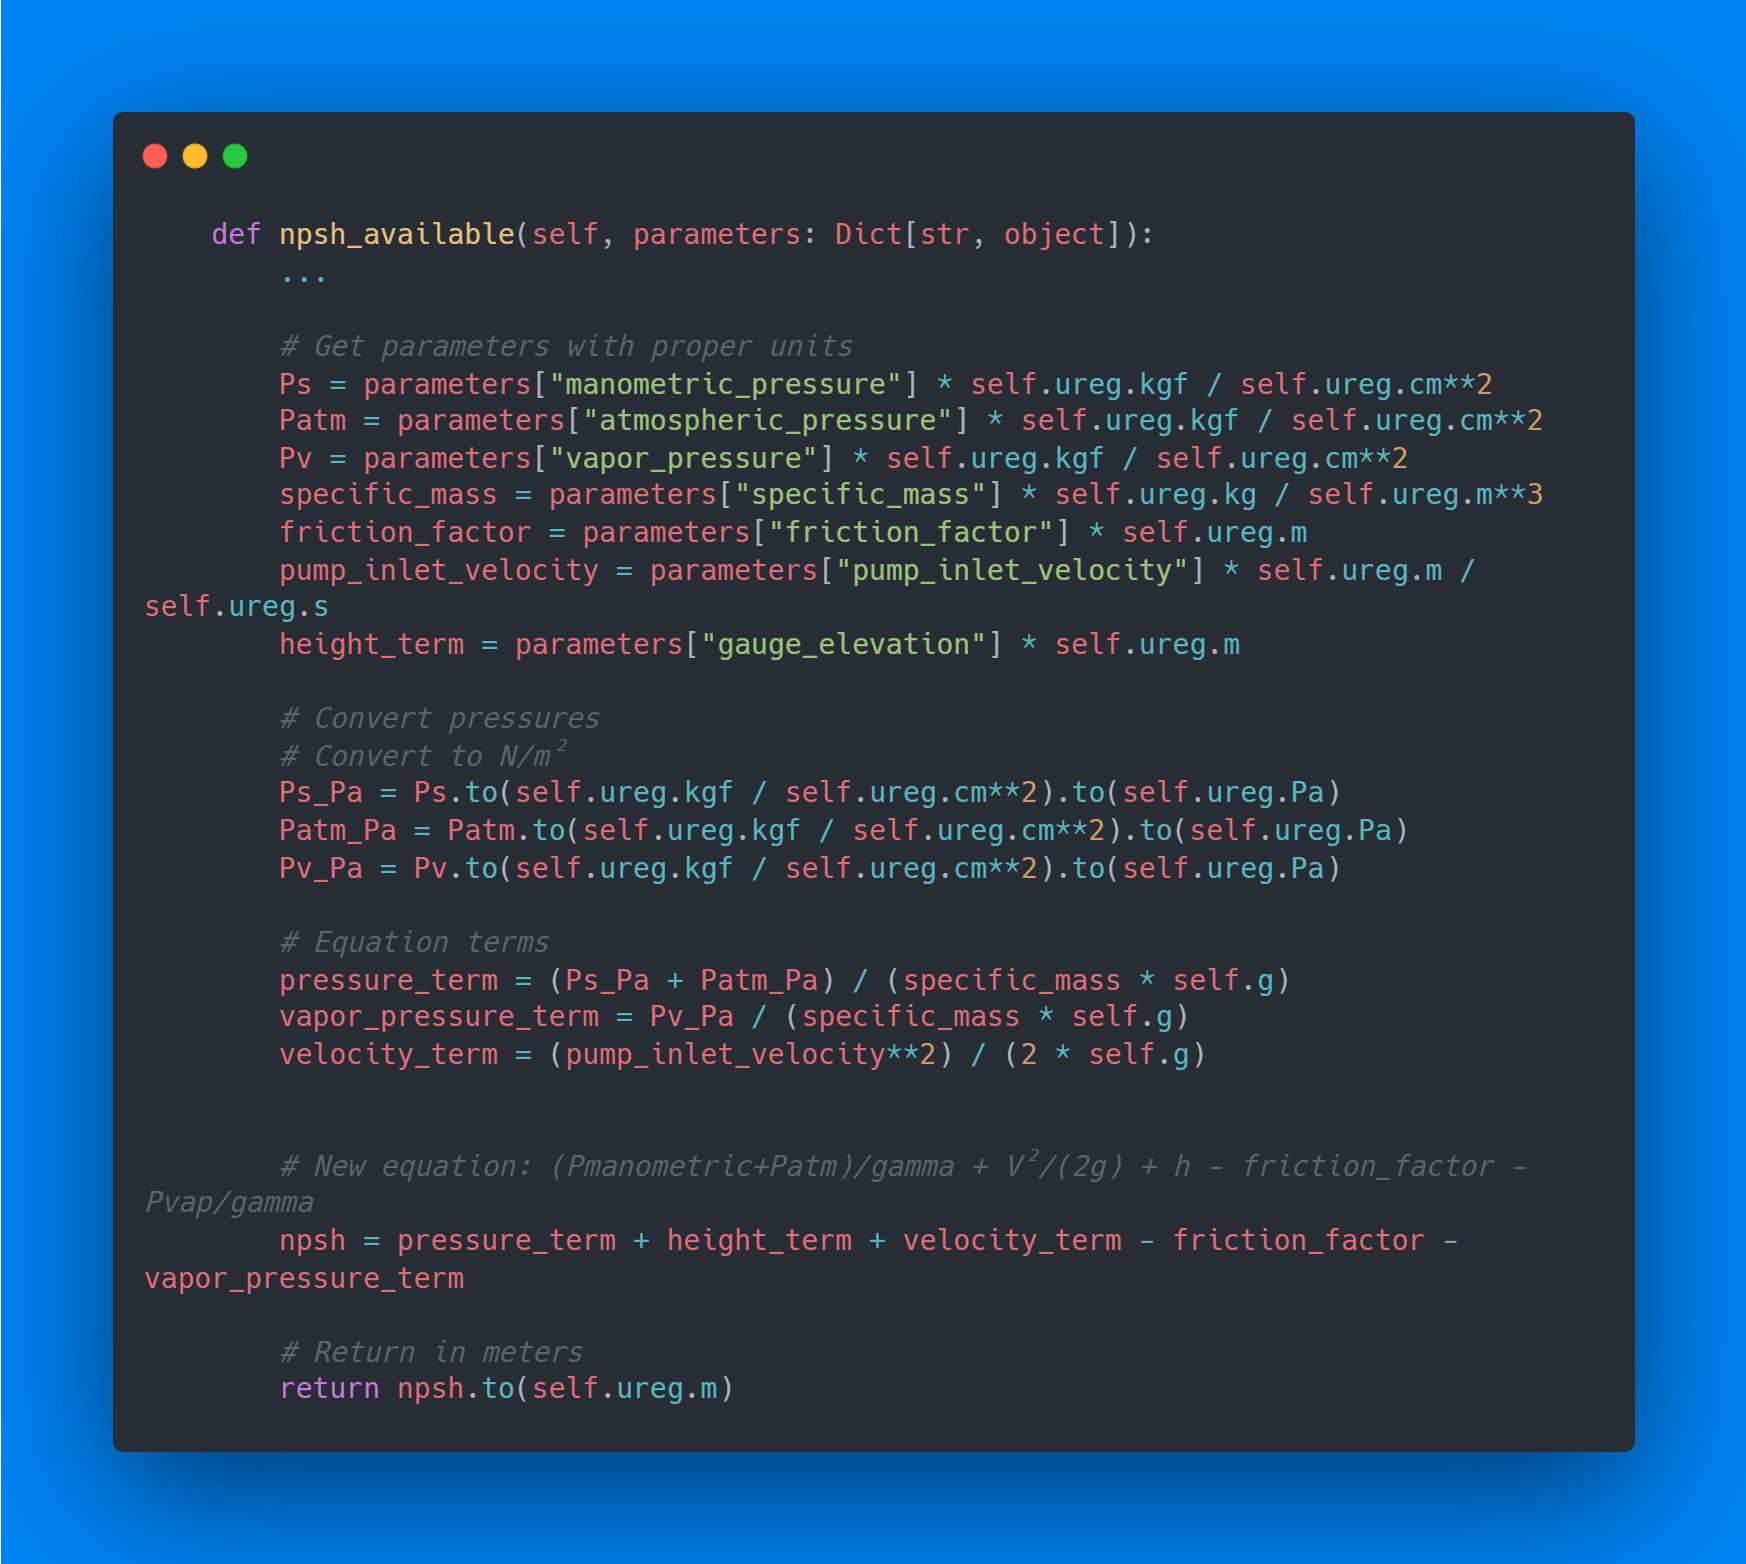
\includegraphics[width=\linewidth]{media/cap4_npsh_parte_dois.png}
    \fonte{Elaboração própria (2026).}
\end{figure}

\subsubsection{Diâmetro Hidráulico para Geometrias Diversas}

O conceito de diâmetro hidráulico generaliza o cálculo do número de Reynolds e do fator de atrito para seções transversais não circulares. O diâmetro hidráulico é definido como:
\begin{equation}
D_{h} = \frac{4 A}{P}
\label{eq:diametro_hidraulico}
\end{equation}
onde $A$ é a área da seção transversal de escoamento e $P$ o perímetro molhado (contorno em contato com o fluido). Assim:

Para dutos circulares, conforme a Equação \ref{eq:dh_circular}:
\begin{equation}
D_{h} = D
\label{eq:dh_circular}
\end{equation}
(recupera o diâmetro interno). Para canais ou abertos, conforme a Equação \ref{eq:dh_rect}:
\begin{equation}
D_{h} = \frac{4 a b}{2 ( a + b )}
\label{eq:dh_rect}
\end{equation}
onde $a$ e $b$ são os lados do retângulo. Para anulares (espaço entre dois tubos concêntricos), conforme a Equação \ref{eq:dh_annular}:
\begin{equation}
D_{h} = D_{o} - D_{i}
\label{eq:dh_annular}
\end{equation}
(diferença entre diâmetro externo interno e diâmetro externo do interno). Para seções triangulares (por ex., condutos abertos triangulares), calcula-se $A$ e $P$ conforme a geometria e aplica-se $4 A / P$. Para geometrias mais complexas (ex.: calhas semicirculares), também se aplica $4 A / P$ considerando o perímetro molhado adequadamente.

\begin{figure}[H]
    \centering
    \caption{Tipos de dutos de escoamento}
    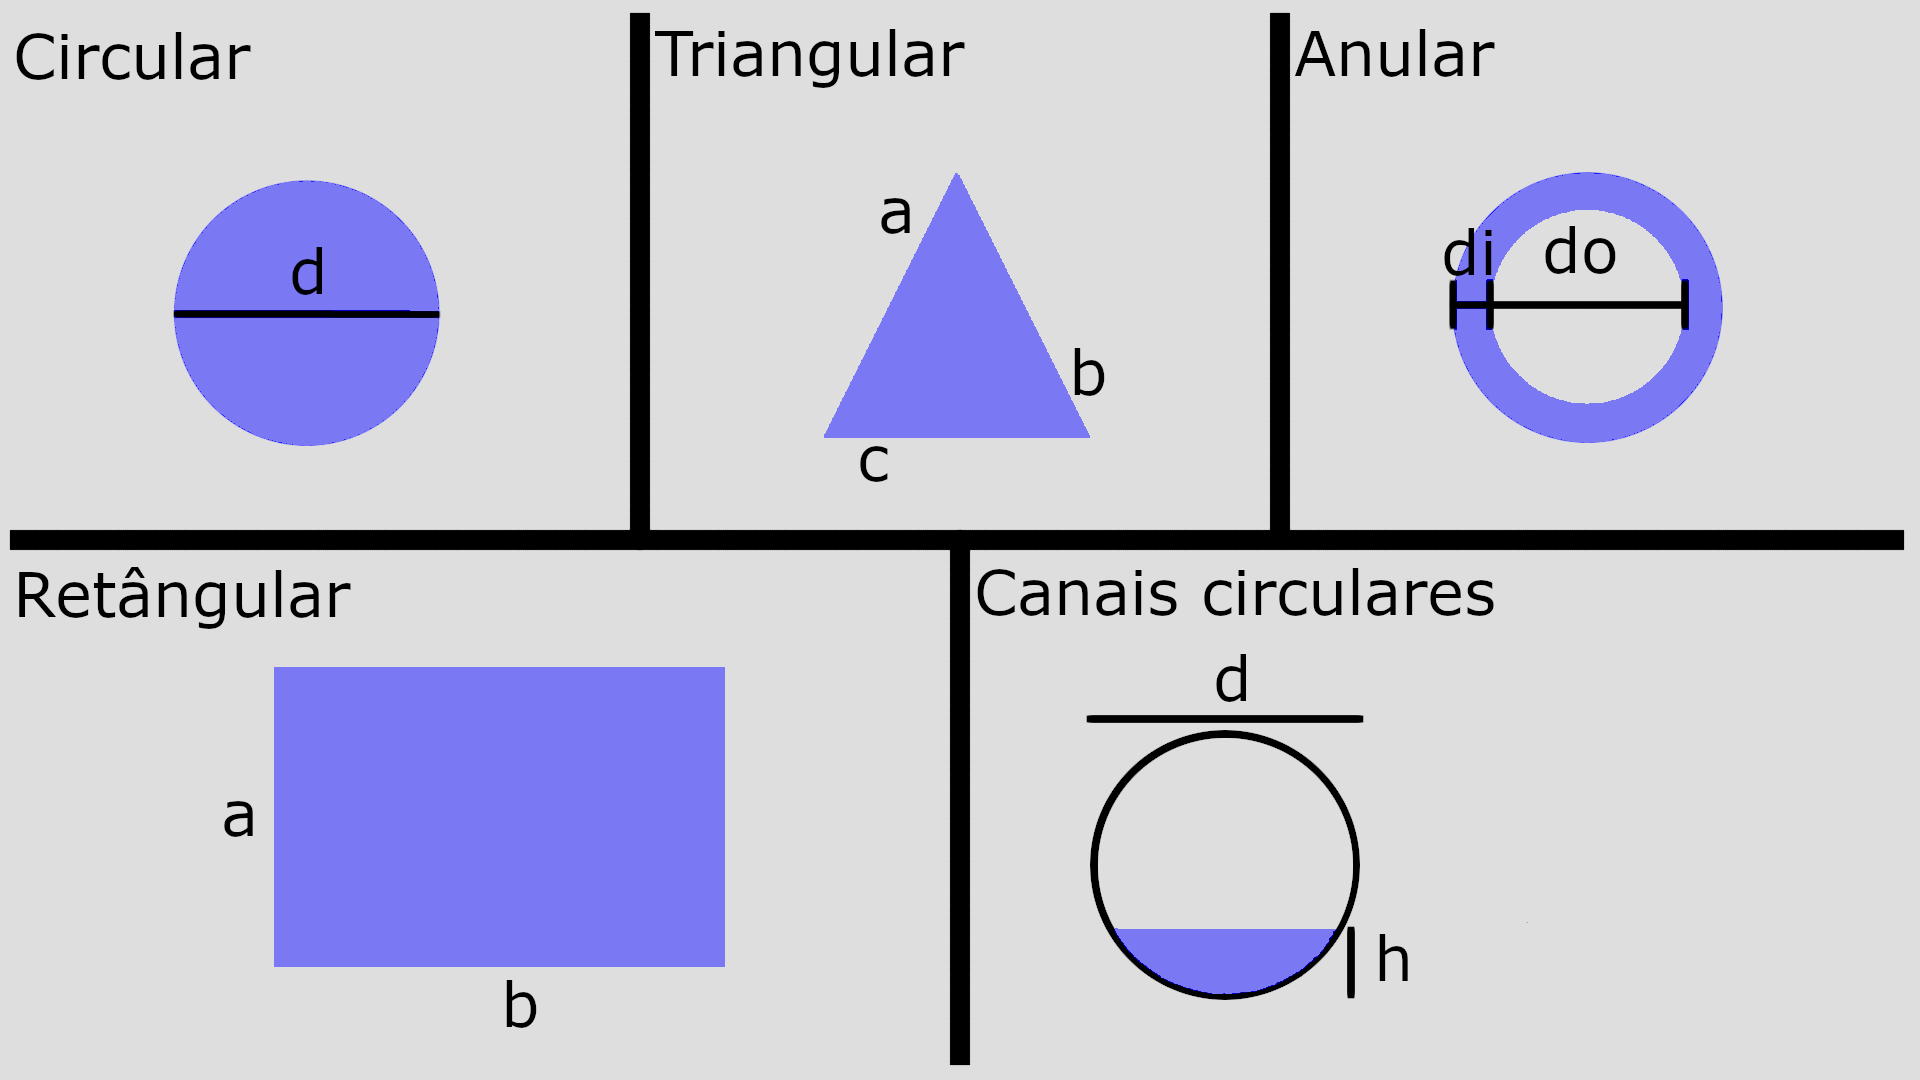
\includegraphics[width=\linewidth]{media/cap4_tipos_dutos_escoamento.png}
    \fonte{Elaboração própria (2026).}
\end{figure}

O programa permite ao usuário informar $A$ e $P$ para cálculo de $D_{h}$ em situações especiais, garantindo flexibilidade para tratar geometrias arbitrárias \cite{white2018}.

\begin{figure}[H]
    \centering
    \caption{Exemplo da identificação e critérios de diâmetro hidráulico}
    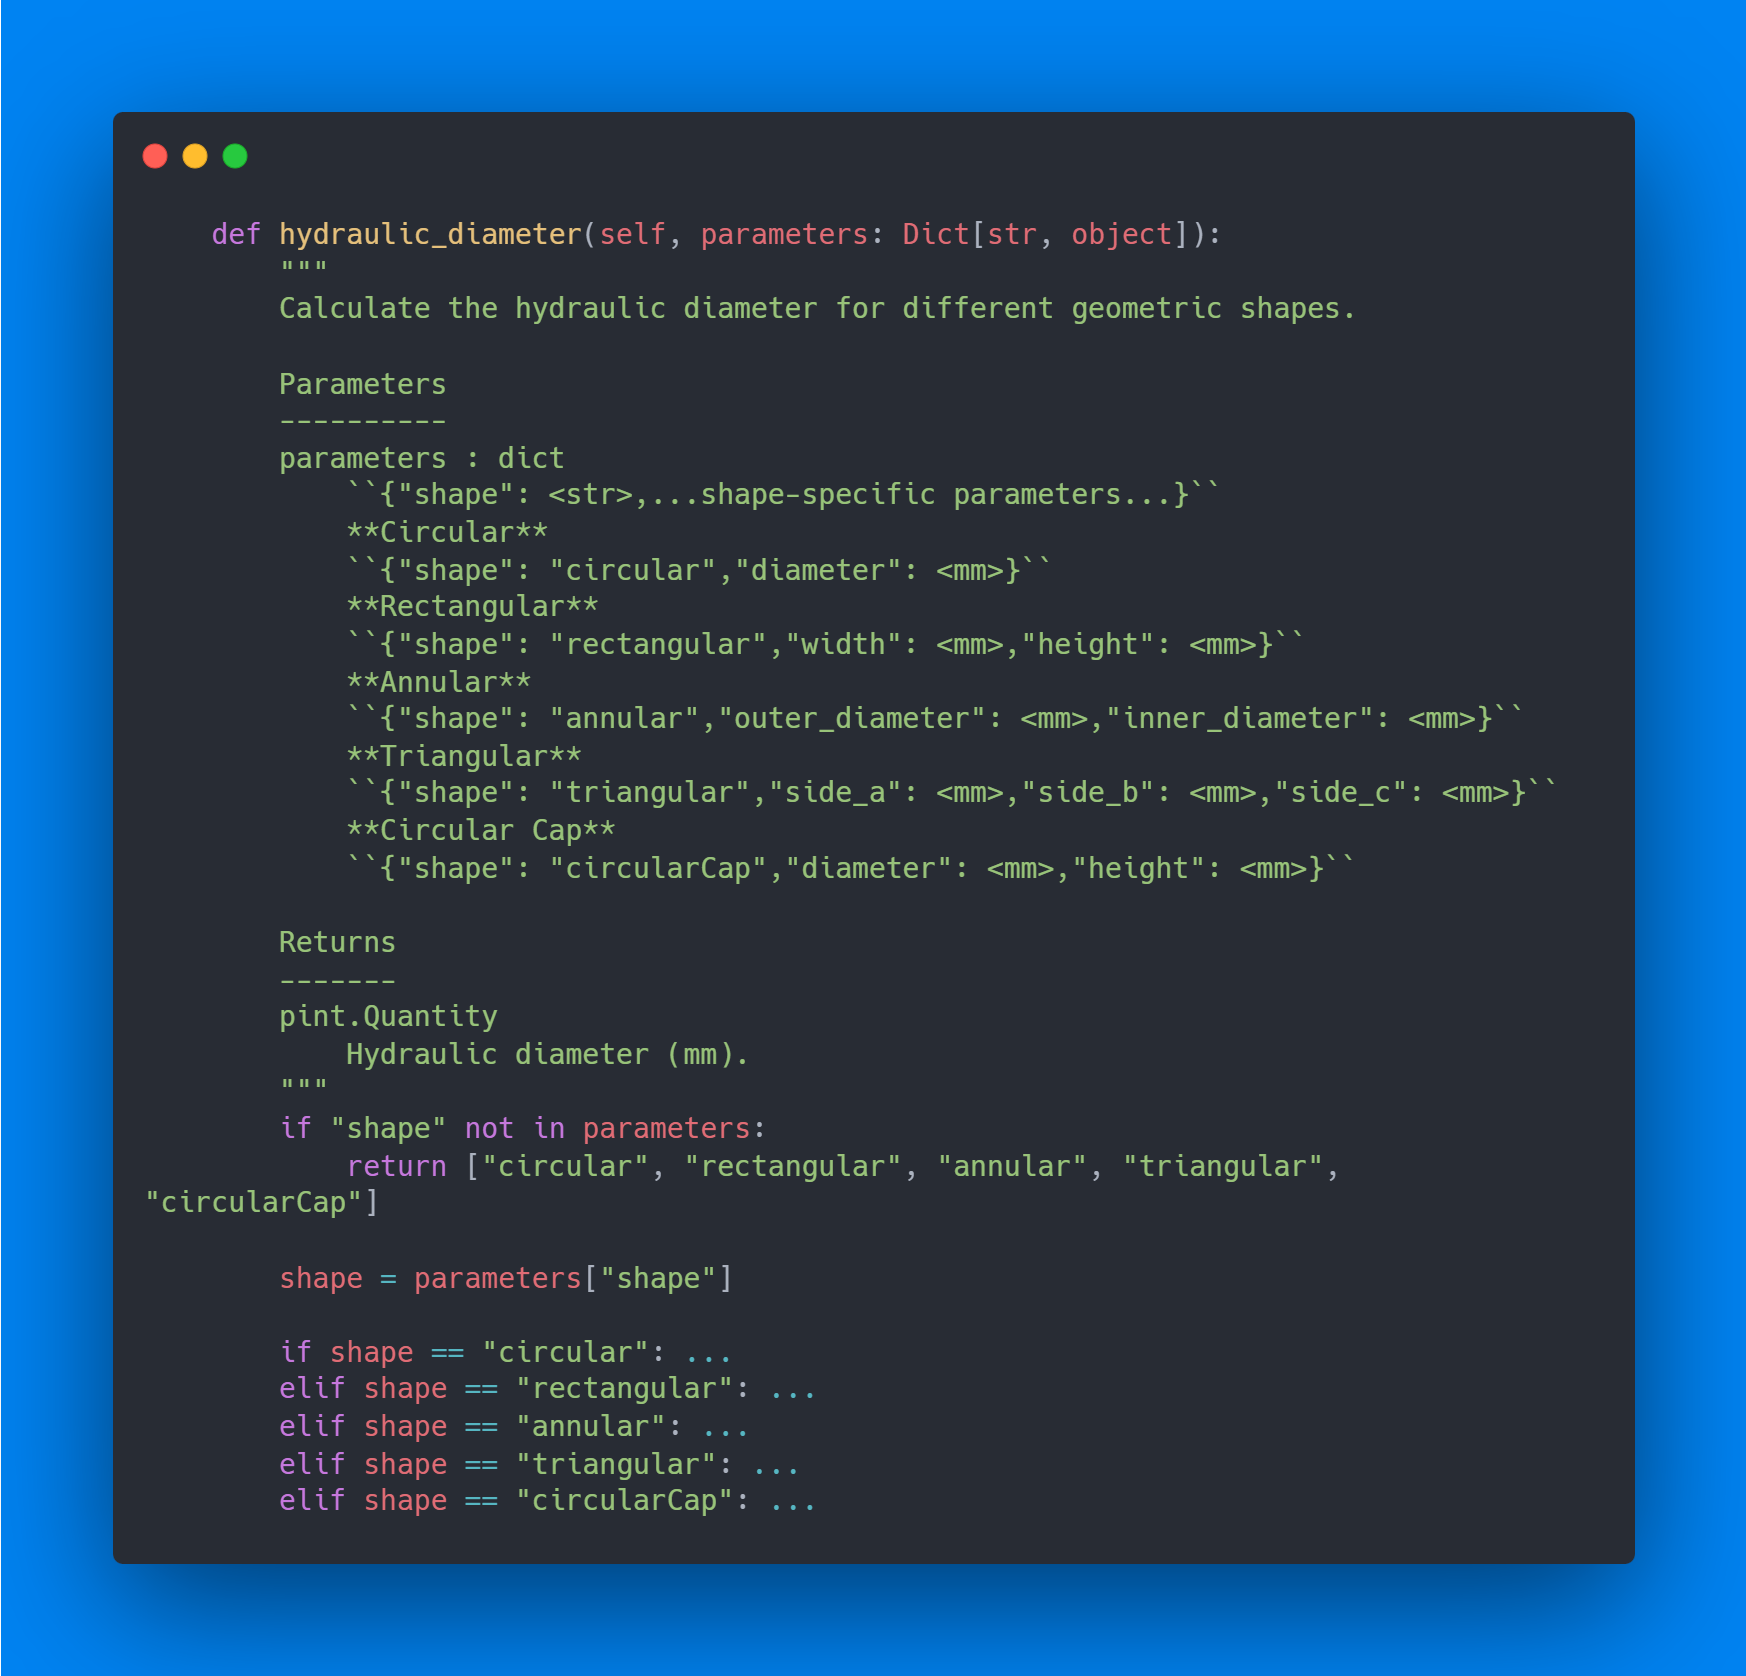
\includegraphics[width=\linewidth,height=0.82\textheight,keepaspectratio]{media/cap4_criterios_diametro_hidraulico.png}
    \fonte{Elaboração própria (2026).}
\end{figure}

\subsection{Propriedades Termofísicas}

Propriedades termofísicas – como massa específica, viscosidade, calor específico, condutividade térmica, entalpia e entropia – são insumos essenciais em praticamente todos os cálculos de processos. Em misturas, a predição de propriedades requer modelos mais complexos do que simples somas ponderadas, considerando interações moleculares e desvios da idealidade. Tais propriedades alimentam balanços de massa e energia, o dimensionamento térmico de trocadores, o cálculo de Reynolds e de fatores de atrito, o desempenho de separações, entre outros. Temperatura e pressão são variáveis determinantes: utilizam-se correlações empíricas (por exemplo, equação de Antoine para pressão de vapor) ou equações de estado (gás ideal, Peng-Robinson, SRK) conforme o sistema. Erros na estimativa de viscosidade ou massa específica afetam o cálculo de Reynolds, fator de atrito e potência de bombeamento; imprecisões em calores específicos ou entalpias propagam-se em balanços de energia e projeto de utilidades.

\begin{figure}[H]
    \centering
    \caption{Obtenção de propriedades pela biblioteca \textit{CoolProp}}
    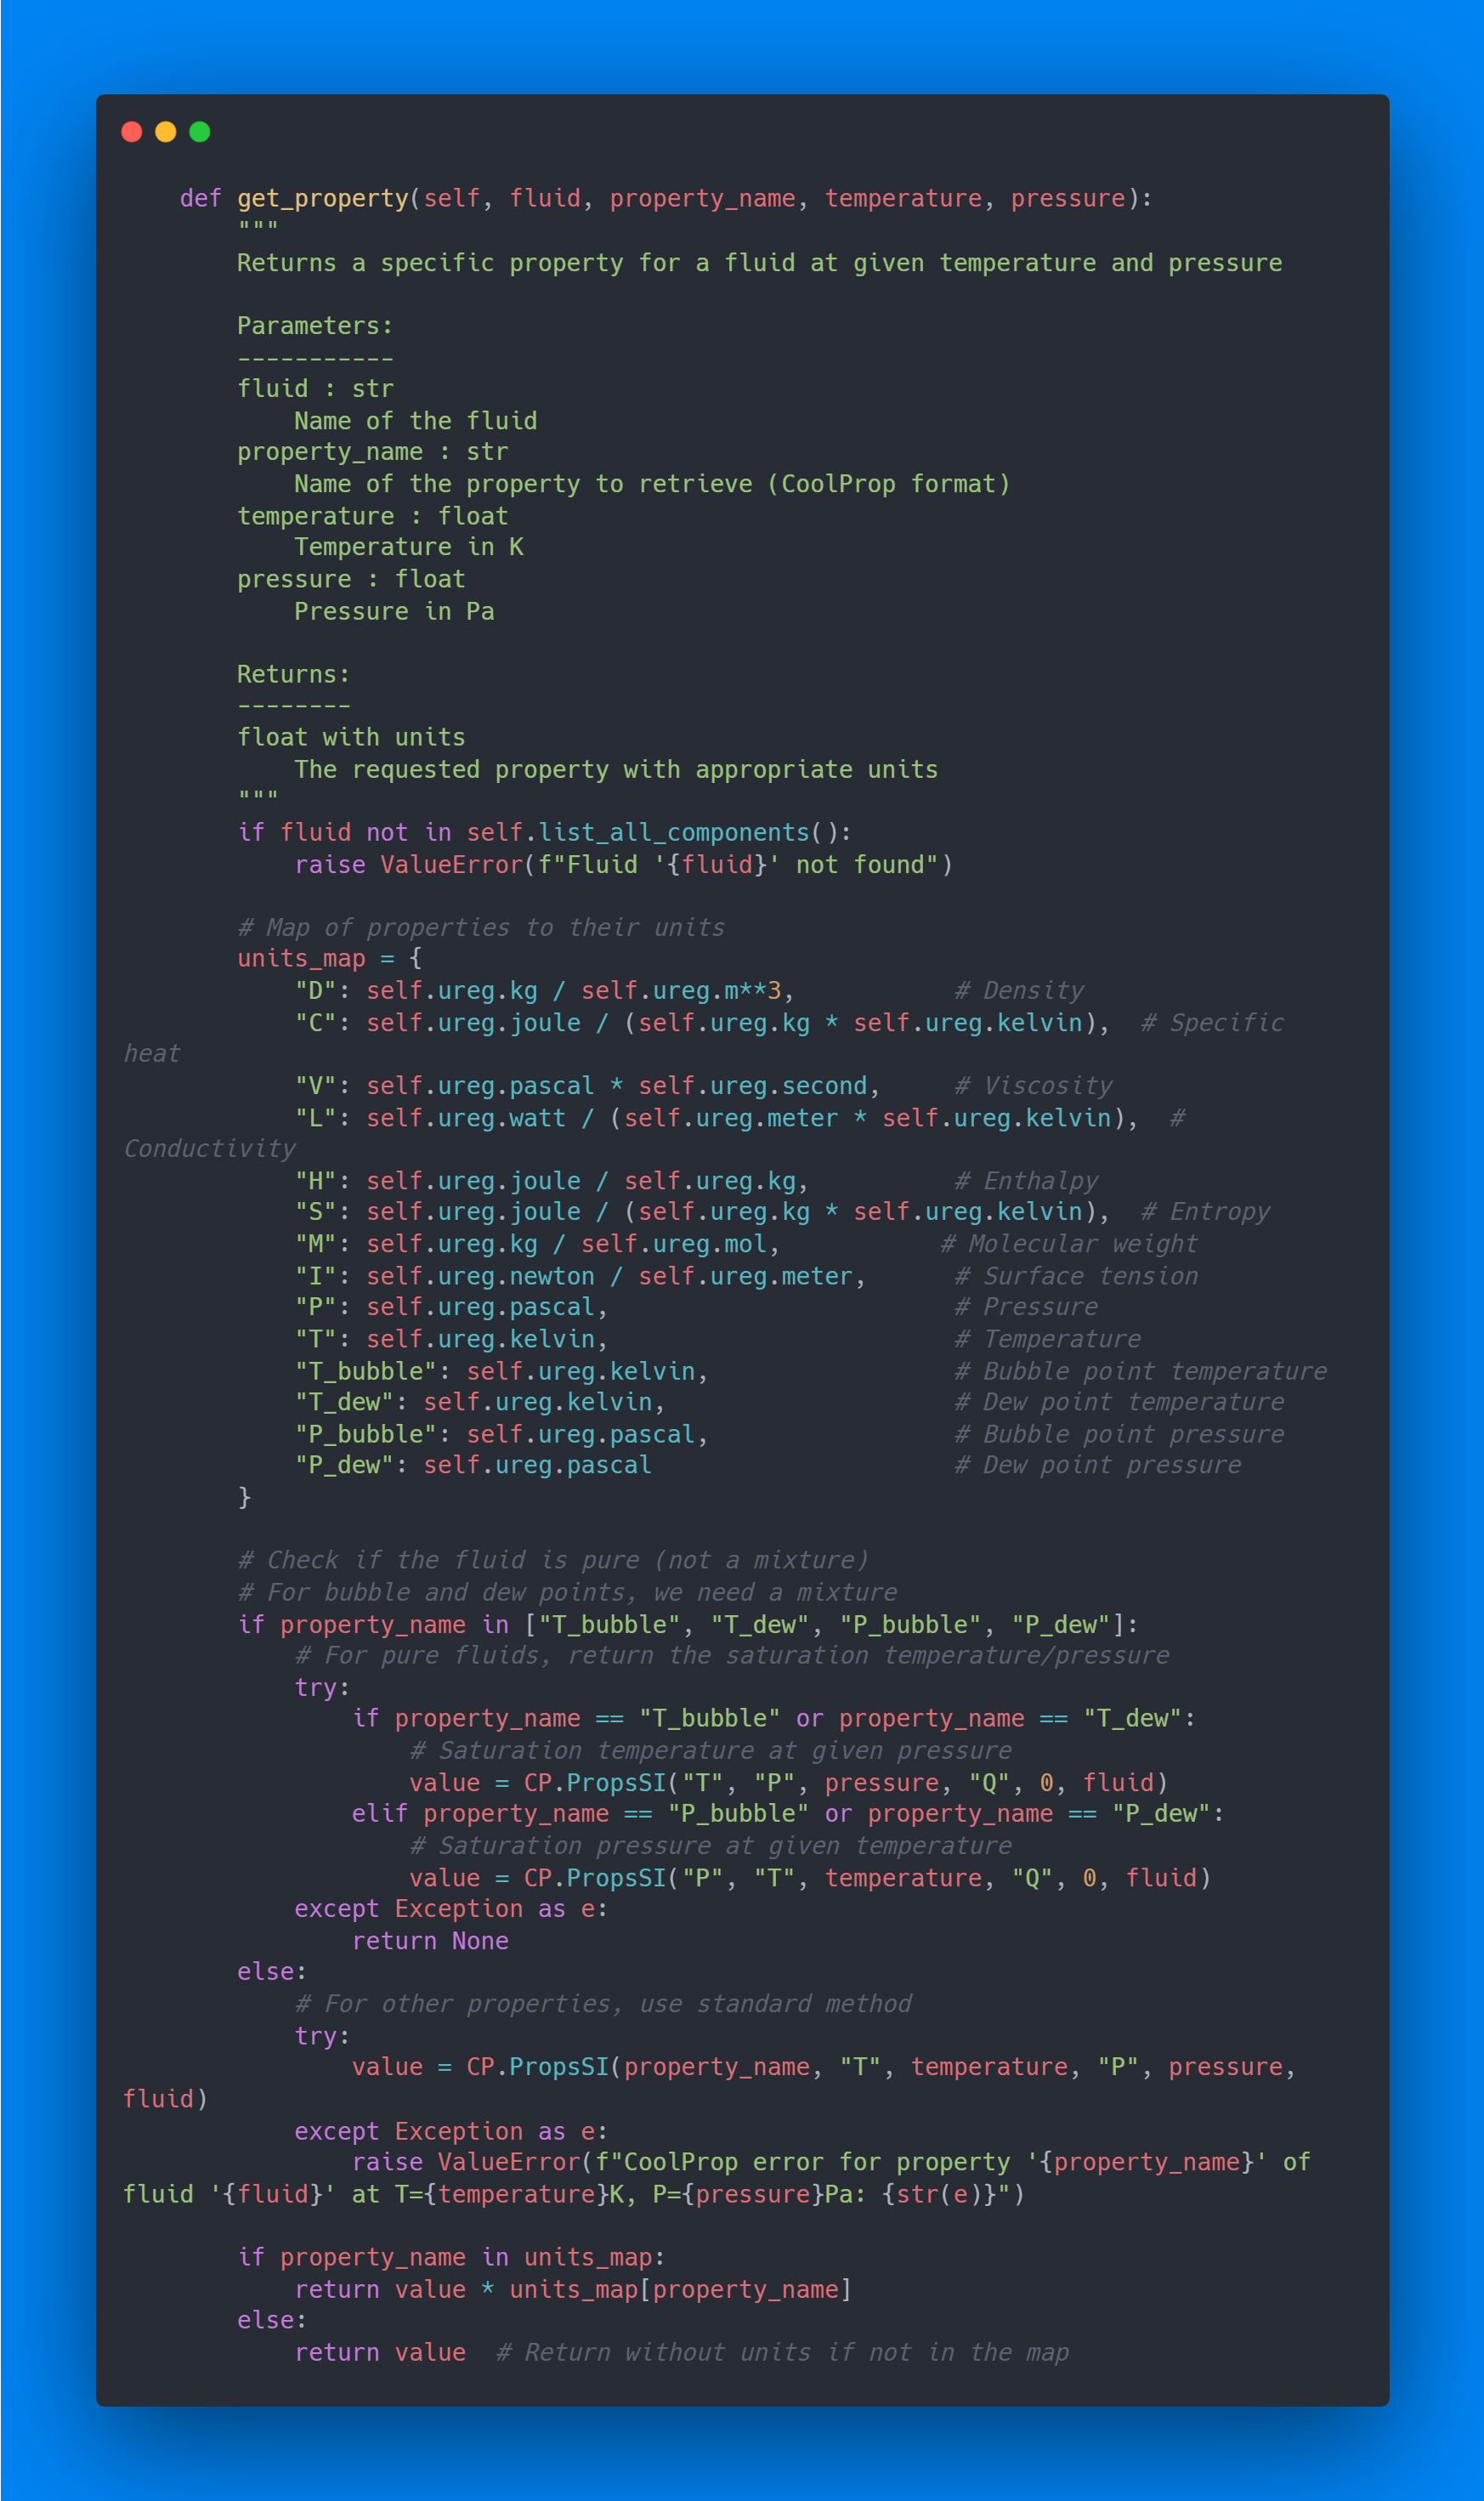
\includegraphics[width=0.9\linewidth,height=0.78\textheight,keepaspectratio]{media/cap4_obtencao_propriedades_coolprop.png}
    \fonte{Elaboração própria (2026).}
\end{figure}

\begin{figure}[H]
    \centering
    \caption{Obtenção de propriedades críticas pela biblioteca \textit{CoolProp}}
    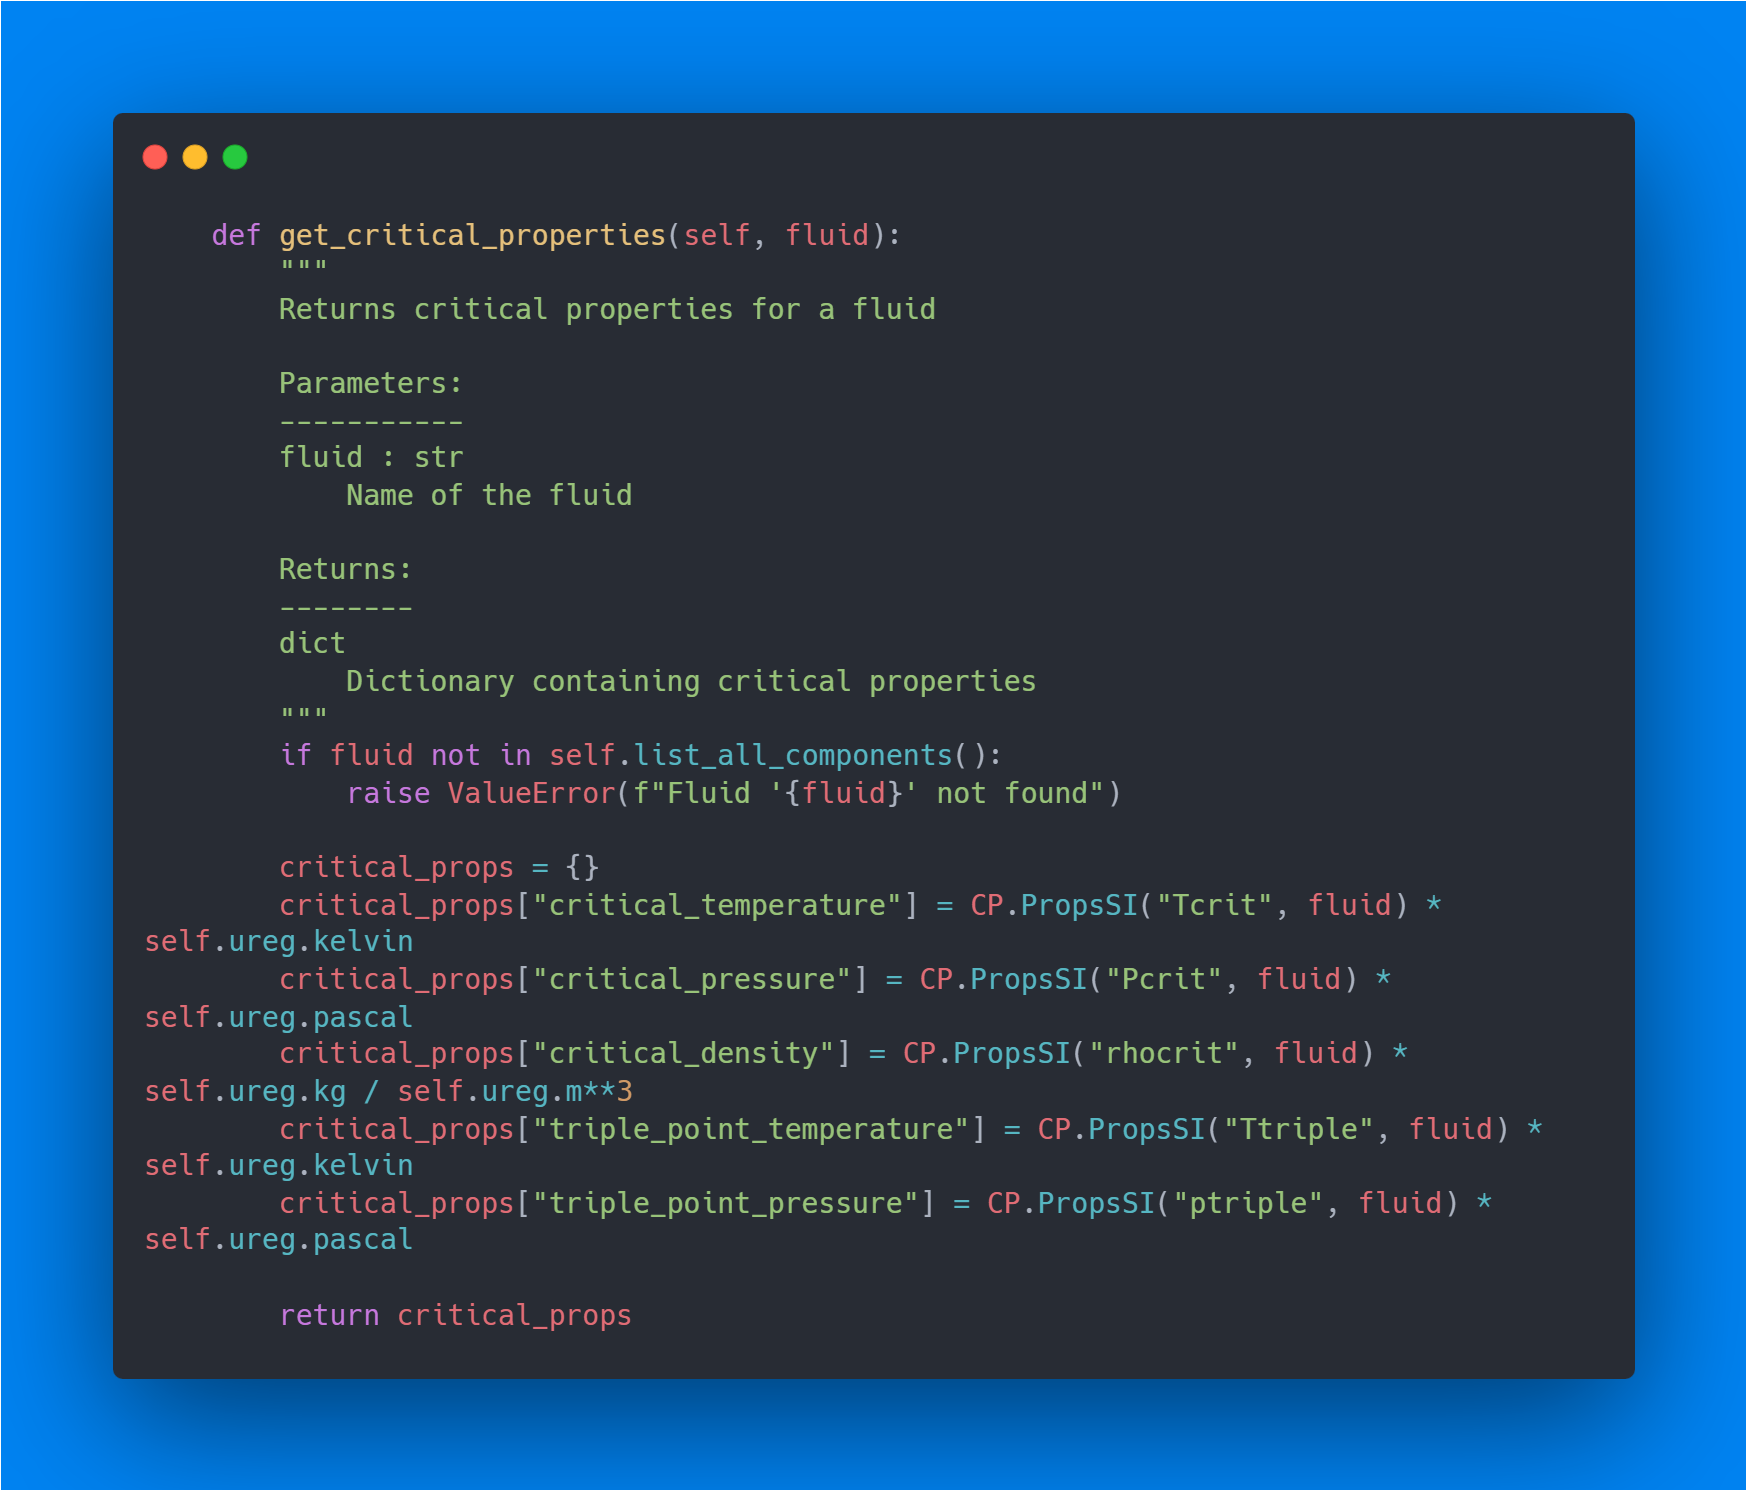
\includegraphics[width=\linewidth]{media/cap4_obtencao_propriedades_criticas_coolprop.png}
    \fonte{Elaboração própria (2026).}
\end{figure}

No \textit{software} desenvolvido, um módulo de propriedades utiliza a biblioteca \textit{CoolProp} para recuperar propriedades de fluidos puros (e misturas) a partir de dados de entrada de $T$ e $P$. São obtidas propriedades como densidade ($\rho$, massa específica), viscosidade, calor específico ($c_{p}$ e $c_{v}$), condutividade térmica, entalpia, entropia, massa molar e tensão superficial, além de propriedades críticas e pontos de saturação (bolha/orvalho) quando aplicável. A visualização desse cálculo de propriedades, com foco no resultado para uma mistura, é apresentada na Figura \ref{fig:mixture_properties}.

\begin{figure}[H]
    \centering
    \caption{Interface de cálculo para as propriedades de uma mistura}
    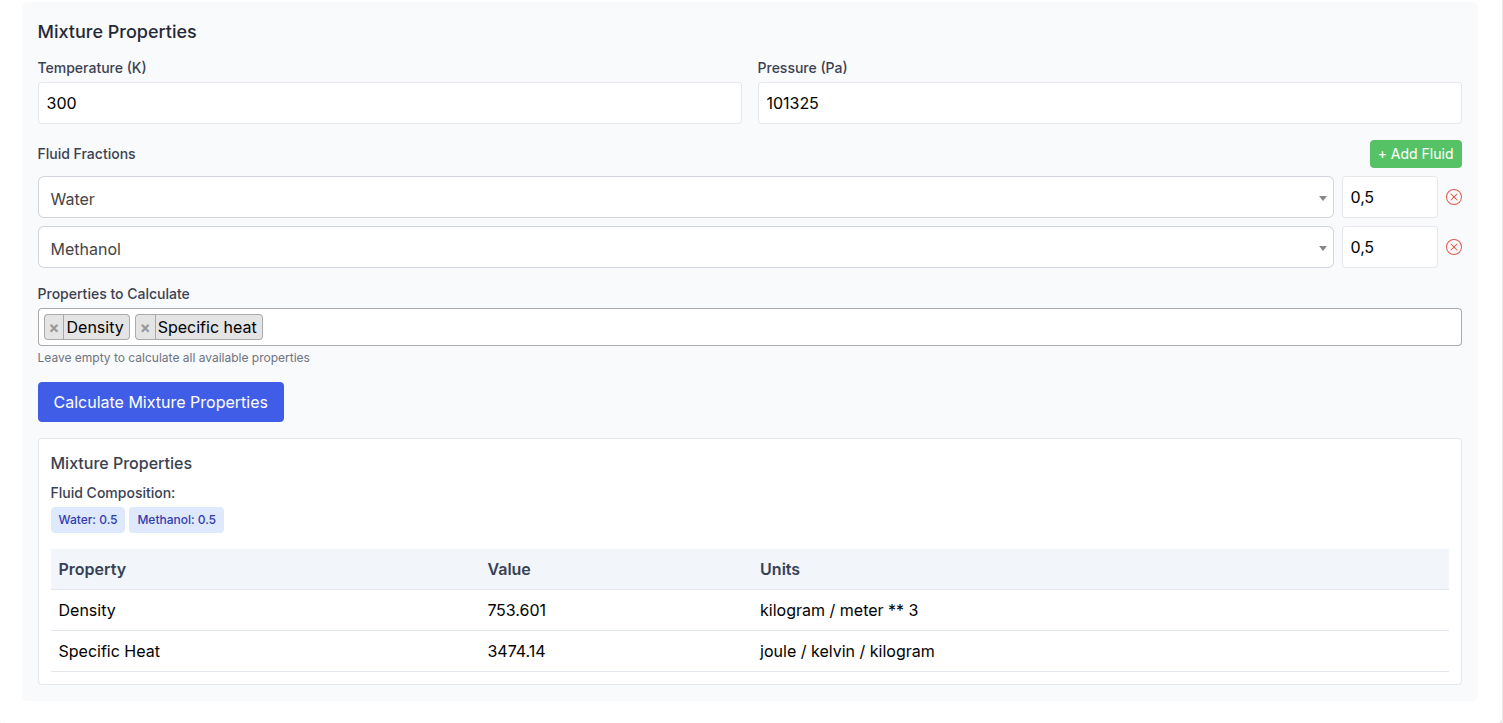
\includegraphics[width=\linewidth]{media/cap4_interface_propriedades_mistura.png}
    \fonte{Elaboração própria (2026).}
    \label{fig:mixture_properties}
\end{figure}

Para misturas, a \textit{API} do \textit{CoolProp} permite montar \textit{strings} com o padrão abaixo, usando as frações especificadas para cada componente \cite{bell2014}:

\begin{quote}
\small\texttt{HEOS::Comp1[x1]\&Comp2[x2]\&...}
\end{quote}

Todas as grandezas retornam já associadas a unidades do SI (via integração com a biblioteca \textit{Pint}), garantindo consistência nos cálculos.

\begin{figure}[H]
    \centering
    \caption{Obtenção de propriedades de misturas pela biblioteca \textit{CoolProp} – Parte 1/2}
    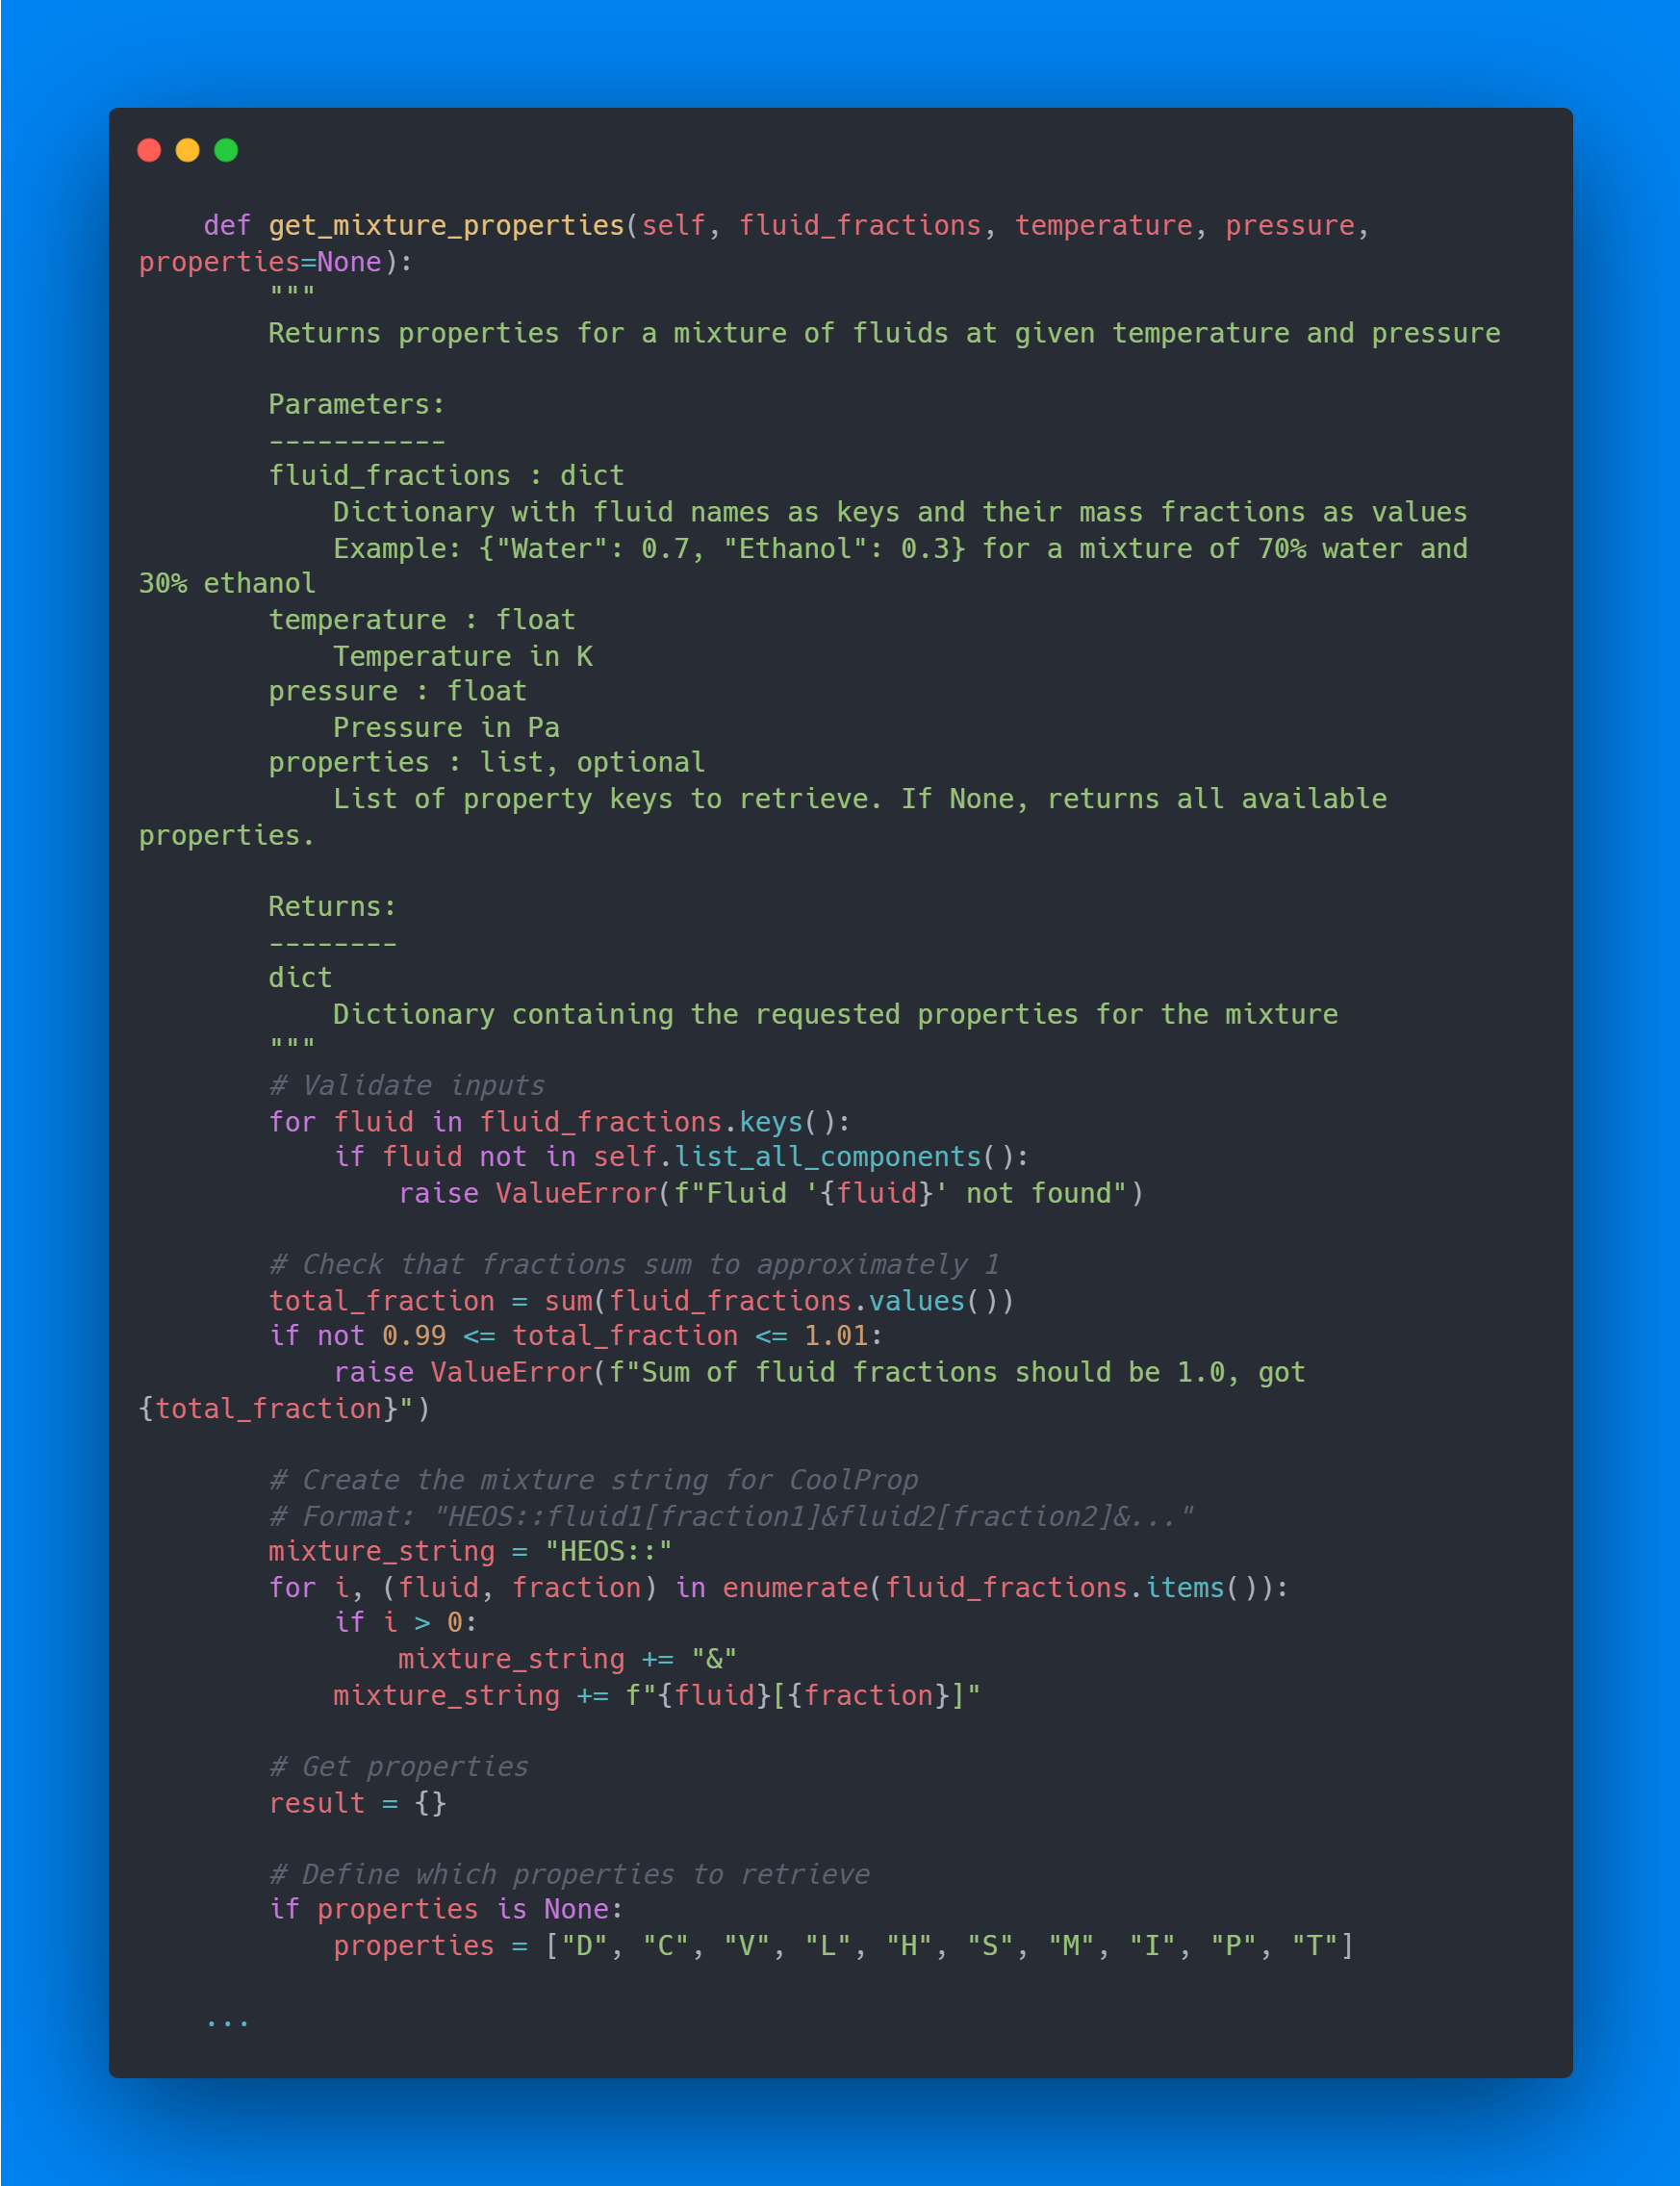
\includegraphics[width=\linewidth]{media/cap4_obtencao_propriedades_misturas_coolprop_parte_um.png}
    \fonte{Elaboração própria (2026).}
\end{figure}

\begin{figure}[H]
    \centering
    \caption{Obtenção de propriedades de misturas pela biblioteca \textit{CoolProp} – Parte 2/2}
    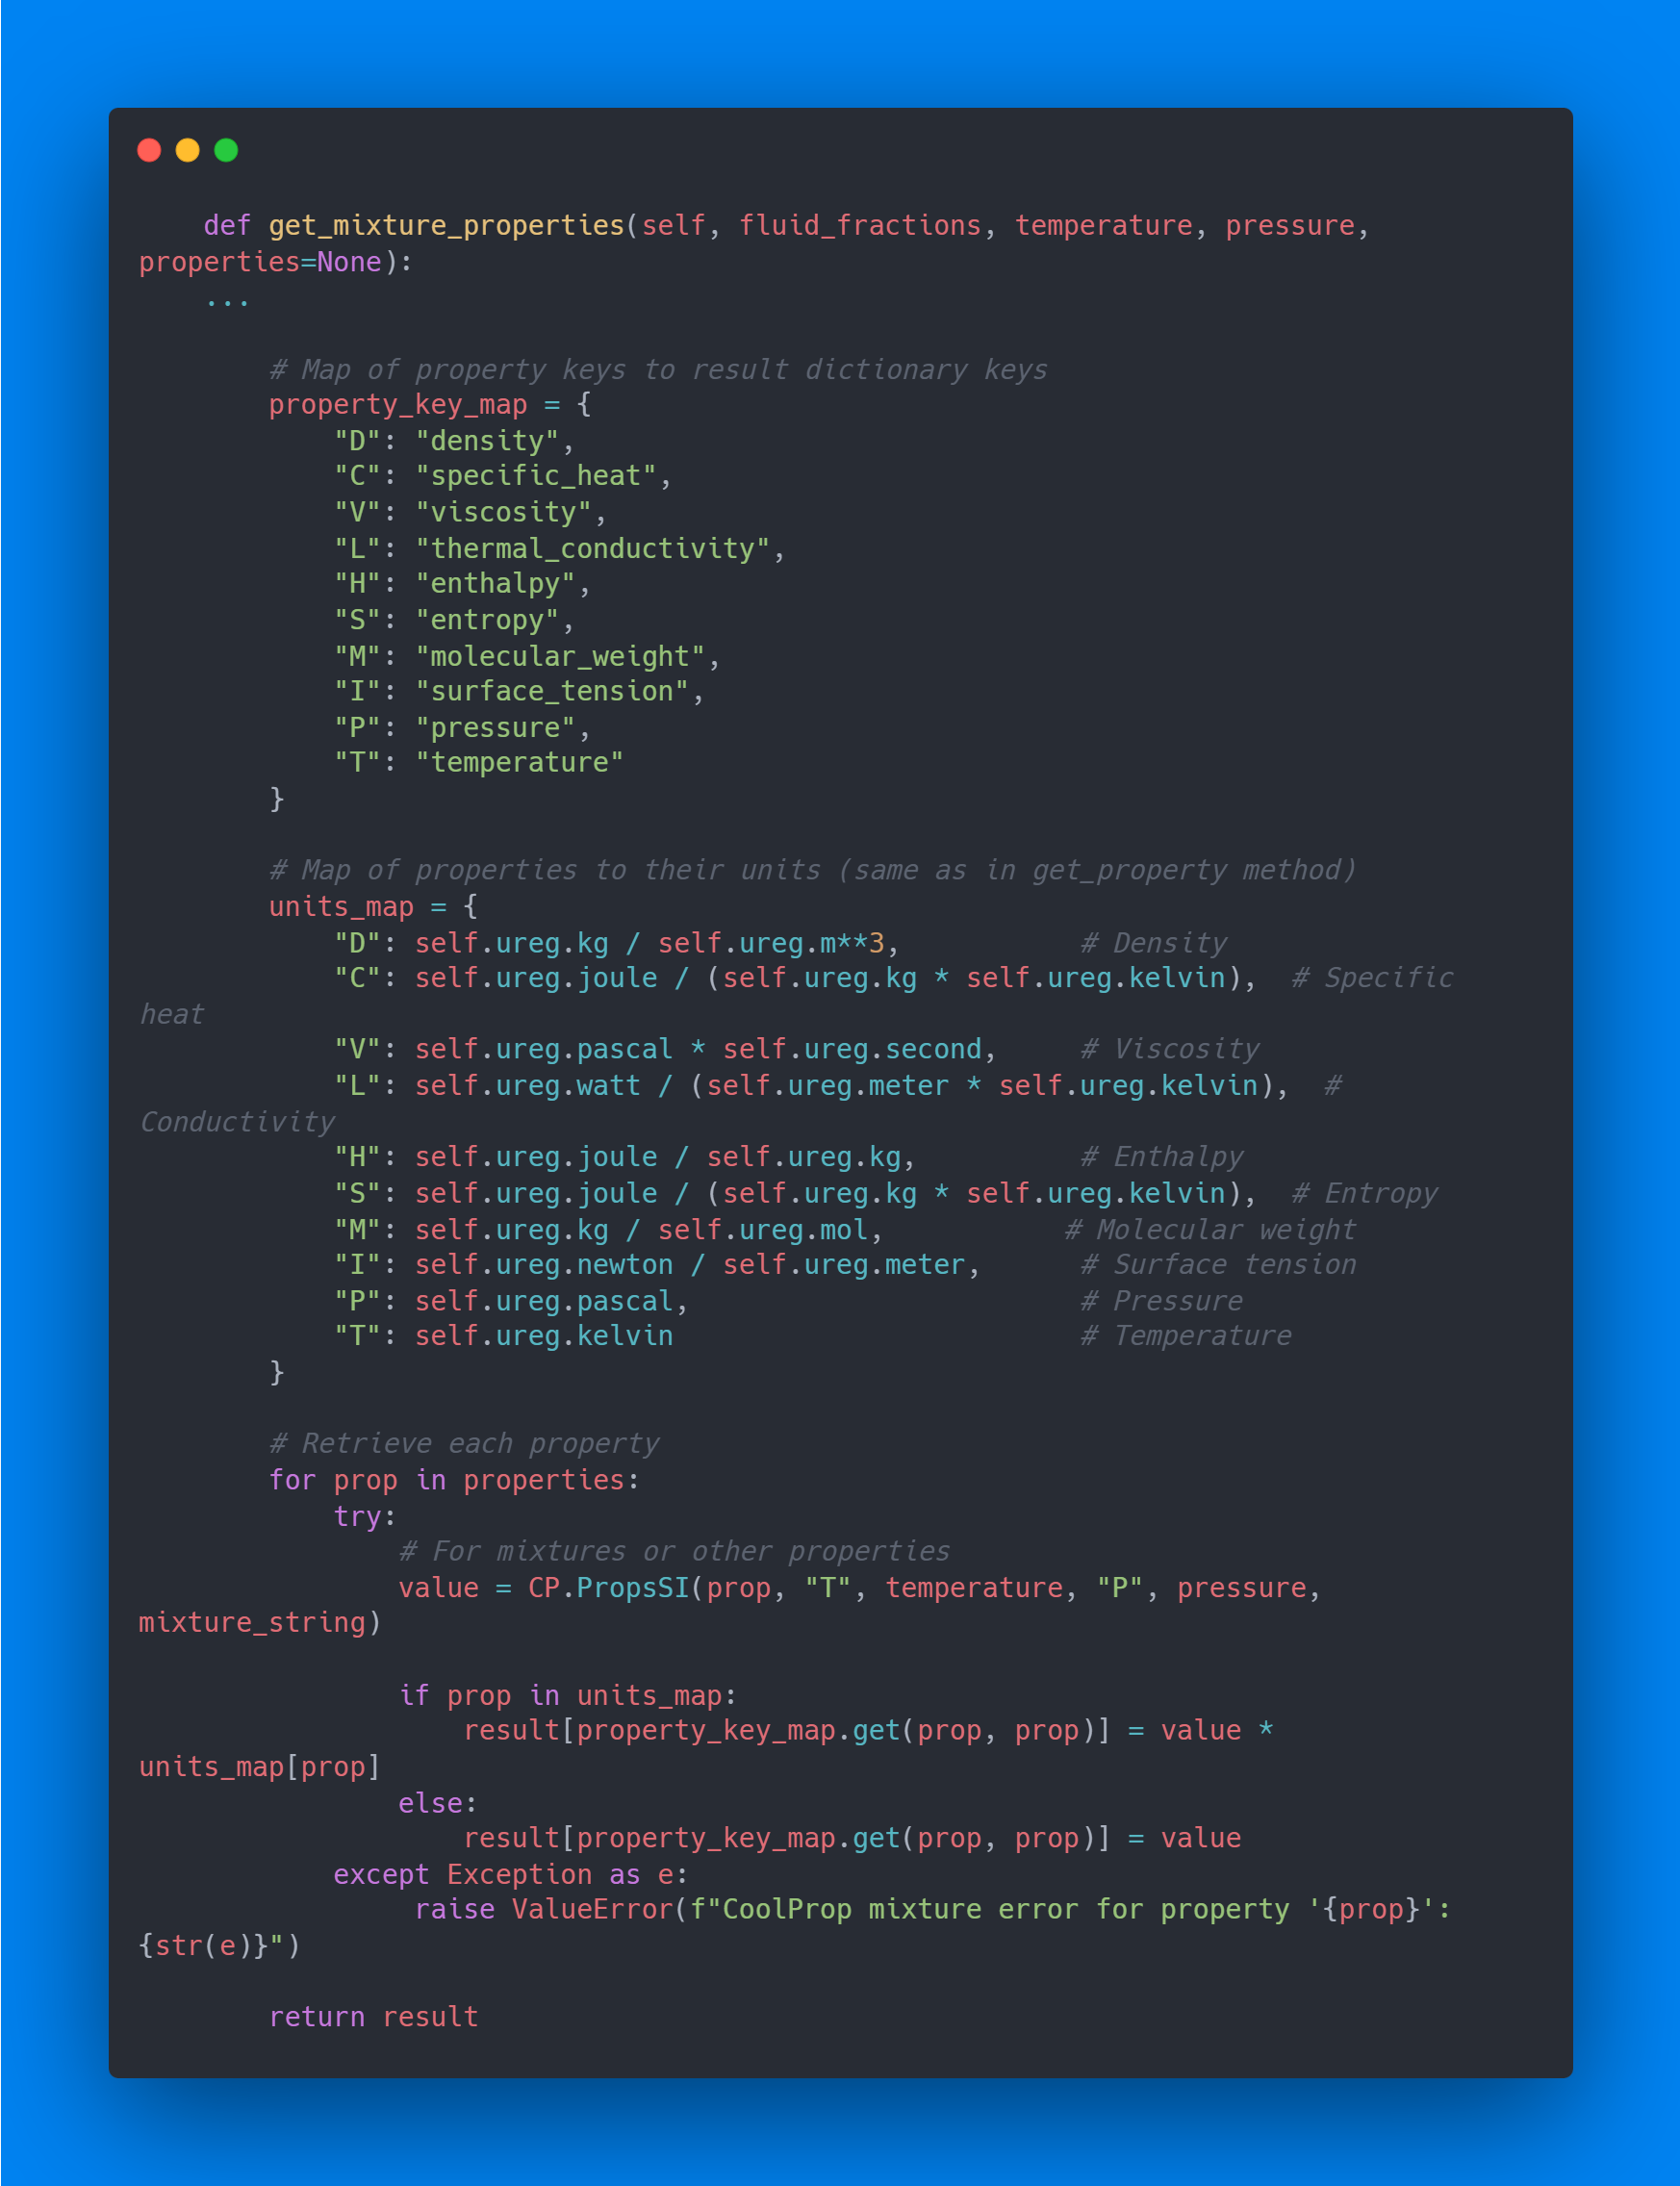
\includegraphics[width=\linewidth]{media/cap4_obtencao_propriedades_misturas_coolprop_parte_dois.png}
    \fonte{Elaboração própria (2026).}
\end{figure}

O uso de uma biblioteca de propriedades de qualidade referência como o \textit{CoolProp} assegura que o \textit{software} tenha um \textit{backend} termodinâmico rigoroso e abrangente, reforçando o caráter didático ao permitir explorar diferentes cenários com fidelidade física.
